\chapter{Models for linear classification}
\label{chap:lin.class}
In this chapter, $Y$ is categorical and takes values in the finite set $\CR_Y = \defset{g_1,
\ldots, g_q}$. The goal is to predict this class variable from the
input  $X$, taking values in a set $\CR_X$. Using the same progression as in the regression case, we will first discuss basic linear methods, for which $\CR_X = \mR^d$ before extending them, whenever possible, to kernel methods, for which $\CR_X$ can be arbitrary as soon as a feature space representation is available. 

Classifiers will be based on a training set $T = ((x_1, y_1), \ldots, (x_N, y_N))$ with $x_k\in\CR_X$ and $y_k\in \CR_Y$ for $k=1, \ldots, N$. For $g\in \CR_Y$, we will also let $N_g$ denote the number of samples in the training set such that $y_k = g$, i.e., 
\[
N_g = \big|\defset{k: y_k=g}\big| = \sum_{k=1}^N \bfone_{y_k=g}.
\]

\section{Logistic regression} 

\subsection{General Framework}
Logistic regression uses the fact that, in order to apply  Bayes's
rule, only the conditional distribution of the class variables $Y$
given $X$ is needed, and trains a parametric model of this distribution. More precisely, if one denotes by $p(g|x)$  the probability that  $Y=g$ conditional to $X=x$, logistic regression assumes that, for some parameters $({a_0}(g), b(g), g\in \CR_Y)$ with ${a_0}(g) \in \mR$ and $b(g)\in \mR^{d}$, one has $p = p_{{a_0},b}$ with 
\[
\log p_{{a_0},b}(g\mid x) = {a_0}(g) +  x^T b(g) - \log(C({a_0}, b, x)),
\]
where
$C({a_0}, b, x) = \sum_{g\in \CR_Y} \exp({a_0}(g) + x^T b(g)).$

Introduce the functions, defined over mappings $\mu: \CR_Y \to \mR$ (which can be identified with vectors in $\mR^q$)  
\begin{equation}
\label{eq:log.reg.F}
F_g(\mu) = \mu(g) - \log \sum_{g'\in \CR_Y} e^{\mu(g')}\,.
\end{equation}
With this notation, letting $\be(g) = \begin{pmatrix}{a_0}(g)\\ b(g)\end{pmatrix}$ and $\tx = \begin{pmatrix}1\\ x\end{pmatrix}$, one has 
$\log p_{\be}(g|x) = F_g(\beta^T\tx)$, where $\beta^T\tx$ is the function $(g'\mapsto \beta(g')^T\tx)$.  

For any constant function $(g \mapsto \mu_0\in \mR)$ one has
\[
F_g(\mu+\mu_0) = \mu(g) +\mu_0 - \log \sum_{g'\in \CR_Y} e^{\mu(g')+\mu_0} =  \mu(g) +\mu_0 - \mu_0 - \log \sum_{g'\in \CR_Y} e^{\mu(g')} = F_g(\mu).
\]
As a consequence, if one replaces, for all $g$,  $\be(g)$ by $\tilde \be(g) = \be(g) + \ga$, with $\ga\in \mR^{d+1}$, then $\tilde \beta^T\tx = \beta^T\tx + \gamma^T\tx$ and
\[
\log p_{\tilde \be}(g\mid x) =   \log p_{\be}(g\mid x).
\]
This shows that the model is over-parametrized. 
 One therefore needs a $(d+1)$-dimensional constraint to ensure uniqueness, and we will enforce a linear constraint in the form
\[
\sum_{g\in \CR_Y} \rho_g \be(g) = c
\]
with $\sum_g\rho_g \neq 0$.



\subsection{Conditional log-likelihood}
The conditional log-likelihood computed from the training set is:
\[
\ell(\be) = \sum_{k=1}^N \log p_\be(y_k\mid x_k)\,.
\]
 Logistic regression computes a maximizer $\hat \be$ of this log-likelihood.
 The classification rule given a new input $x$ then chooses the class $g$ for which $p_{\hat \be}(g\mid x)$ is largest, or, equivalently, the class $g$ that maximizes $\tx^{T} \be(g)$.
 
\begin{proposition}
\label{prop:log.reg}
Let  $\tm_{g} = \sum_{k:y_{g}=k} x_{k}/N_{g}$.
The conditional log-likelihood $\ell$ is concave with first derivative
\begin{equation}
\label{eq:log.reg.d1}
\prt_{\beta(g)} \ell  = N_{g} \tm^{T}_{g} -\sum_{k=1}^{N} 
\tilde x_{k}^T p_\be(g|x_{k})
\end{equation}
and negative semi-definite second derivative
\begin{equation}
\label{eq:log.reg.d2}
\prt_{\beta(g)}\prt_{\beta(g')} \ell =  -\bfone_{[g=g']}\sum_{k=1}^{N}\tilde x_{k} \tilde x_{k}^T
 p_\be(g|x_{k}) + \sum_{k=1}^{N}
\tilde x_{k} \tilde x^T_{k} p_\be(g|x_{k}) p_\be(g'|x_{k})\,.
\end{equation}
\end{proposition}
\begin{remark}
\label{rem:log.reg.notation}
In this discussion, we consider $\ell$ as a function defined over collections $(\beta(g), g\in \CR_Y)$, or, if one prefers, on the $q(d+1)$-dimensional linear space, $\CF$, of functions $\beta: \CR_Y \to \mR^{q+1}$. With this in mind, the differential $d\ell(\beta)$ is a linear form from $\CF$ to $\mR$, therefore associating to any family $u = (u(g), g\in\CR_Y)$, the expression
\[
d\ell(\beta) \,u = \sum_{g\in\CR_Y} \prt_{\beta(g)} \ell\, u(g).
\]
Similarly, the second derivative is the bilinear form
\[
d^2\ell(\beta)(u,u') = \sum_{g, g'\in\CR_Y} u(g)^T \prt_{\beta(g)}\prt_{\beta(g')}\ell \, u(g').
\]
The last statement in the proposition expresses the fact that $d^2\ell(\beta)(u,u) \leq 0$ for all $u\in\CF$.
\end{remark}
\begin{proof}
First consider the function $F_g$ in \cref{eq:log.reg.F}, so that 
\[
\ell(\beta) = \sum_{k=1}^N F_{y_k}(\beta^T\tx_k).
\]
We have, for $\zeta: \CR_Y\to \mR$, 
\[
dF_g(\mu)\zeta =  \zeta(g) - \frac{\sum_{g'\in \CR_Y} e^{\mu(g')} \zeta(g')}{\sum_{g'\in \CR_Y} e^{\mu(g')}}
\]
as can be easily computed by evaluating the derivative of $F(\mu+\epsilon u)$ at $\epsilon=0$. Introducing the notation
\[
q_\mu(g) = \frac{e^{\mu(g)}}{\sum_{g\in \CR_Y} e^{\mu(g)}}
\]
and
\[
\langle \zeta \rangle_\mu = \sum_{g\in \CR_Y} \zeta(g) q_\mu(g),
\]
we have $dF_g(\mu)\zeta =  \zeta(g) - \langle \zeta \rangle_\mu $. 
Evaluating the derivative of $dF_g(\mu+\epsilon u')(\zeta)$ at $\epsilon=0$, one gets (the computation being left to the reader)
\begin{equation}
\label{eq:d2.Fg}
d^2F_g(\mu)(\zeta, \zeta') =   - \langle \zeta \zeta' \rangle_\mu + \langle \zeta \rangle_\mu \, \langle \zeta' \rangle_\mu.
\end{equation}
Note that $-d^2F_g(\mu)(\zeta, \zeta)$ is the variance of $\zeta$ for the probability mass function $q_\mu$ and is therefore non-negative (so that $F_\mu$ is concave). This immediately shows that $\ell$ is concave as a sum of concave functions.  



Using the chain rule, we have, for $u:\CR_Y\to \mR^q$,
\[
d\ell(\beta)u = \sum_{k=1}^N dF_{y_k}(\beta^T\tx_k)\tx_k^Tu(\cdot) = \sum_{k=1}^N \tx_k^Tu(y_k) - \sum_{k=1}^N \langle \tx_k^T u(\cdot) \rangle_{\beta^T\tx_k}.
\]
Reordering the first sum in the right-hand side according to the values of $y_k$ gives
\[
\sum_{k=1}^N u(y_k)^T\tx_k = \sum_{g\in\CR_Y} N_g u(g)^T \tm_g.
\]
Noting that $q_{\beta^T\tx} = p_\beta(\cdot|x)$, we find
\[
d\ell(\beta)(u) =  \sum_{g\in\CR_Y} N_g \tm_g^T u(g) - \sum_{g\in\CR_Y} \tx_k^Tu(g) p_\beta(g|x_k),
\]
yielding \cref{eq:log.reg.d1}. Applying the chain rule again, we have
\begin{equation}
\label{eq:d2.ell.F}
d^2\ell(\beta)(u, u') = \sum_{k=1}^N d^2F_{y_k}(\beta^T\tx_k)(\tx_k^Tu(\cdot), \tx_k^Tu'(\cdot))
\end{equation}
with
\begin{align*}
d^2F_{y_k}(\beta^T\tx_k)(\tx_k^Tu(\cdot), \tx_k^Tu'(\cdot)) =& - \langle u(\cdot)^T \tx_k\tx_k^T u'(\cdot)  \rangle_{\beta^T\tx_k} + \langle \tx_k^Tu(\cdot) \rangle_{\beta^T\tx_k} \, \langle \tx_k^Tu'(\cdot) \rangle_{\beta^T\tx_k}\\
 =& - \sum_{g\in \CR_Y} u(g)^T \tx_k\tx_k^T u'(g) p_\beta(g|x_k) \\
& + \sum_{g,g'\in\CR_Y} u(g)^T \tx_k\tx_k^T u'(g') p_\beta(g|x_k) p_\beta(g'|x_k)
\end{align*}
from which \cref{eq:log.reg.d2} follows.
\end{proof}

\begin{remark}
From $F_g(\mu + \mu_0) = F_g(\mu)$ when $\mu_0$ is constant on $\CR_Y$, one deduces (taking the derivative at $\mu_0 = 0$) that $dF_g(\mu) \boldsymbol 1 = 0$ for all $\mu$, where $\boldsymbol 1$ denotes the constant function equal to 1 on $\CR_Y$. For $h\in \mR^{d+1}$, let $\mathbb c_h$ denote the constant function $\mathbb c_h(g) = h$, $g\in \CR_Y$. We have
\[
d\ell(\beta)\,  \mathbb c_h  =  \sum_{k=1}^N dF_{y_k}(\beta^T\tx_k)\tx_k^T\mathbb c_h =  \sum_{k=1}^N dF_{y_k}(\beta^T\tx_k)(\tx_k^Th \boldsymbol 1) = \sum_{k=1}^N (\tx_k^Th) dF_{y_k}(\beta^T\tx_k) \boldsymbol 1  = 0.
\]
Taking one extra derivative we see that 
\[
d\ell(\beta) (\mathbb c_h , u) = 0
\]
for all functions $u: \CR_Y \to \mR^q$.
\end{remark}

We now discuss whether there are other elements in the null space of the second derivative of $\ell$. We will use notation introduced in the proof of \cref{prop:log.reg}.  From \cref{eq:d2.Fg}, we have $d^2F_g(\mu)(\zeta, \zeta) = 0$ if and only if the variance of $\zeta$ for $q_\mu$ vanishes, which, since $q_\mu >0$, is equivalent to $\zeta$ being constant. So, the null space of $d^2F_g(\mu)$ is one-dimensional, and composed of scalar multiples of $\boldsymbol 1$. Using \cref{eq:d2.ell.F}, we see that $d^2\ell(u,u) = 0$ if and only if , for all $k=1, \ldots, N$, $(g\mapsto \tx_{k}^{T} u(g))$ is a constant function.
 
Assume that  this is true. Then, 
letting $\bar u = \frac1q \sum_{g\in\CR_Y}  u(g)$, one has, for all $g\in\CR_Y$ and $k=1, \ldots, N$,
\[
\tx_{k}^{T} u(g) = \tx_{k}^{T} \bar u
\]
so that $u(g) - \bar u$ is in the null space of the matrix $\CX$. This leads to the following proposition.
\begin{proposition}
\label{prop:log.reg.hess}
Assume that $\CX$ has rank $d+1$. Then the null space of $d^2\ell(\beta)$ is the set of all vectors $u =\mathbb c_h $ for $h\in\mR^{d+1}$. In particular, for any $c\in\mR^{d+1}$, the function $\ell$ restricted to the space
\[
M = \defset{ \be: \sum_{g\in \CR_Y} \rho_g \be(g) = c}
\]
is strictly concave as soon as the scalar coefficients $(\rho_g, g\in\CR_Y)$ are such that $\sum_{g\in\CR_Y} \rho_g \neq 0$.
\end{proposition}
\begin{proof}
From the discussion before the proposition, $u\in \mathrm{Null}(d^2\ell)$ implies that $\CX(u(g) - \bar u) =0$ for all $g$, and since we assume that $\CX$ has rand $d+1$, this requires that $u(g) = \bar u$ for all $g$, i.e., $u = \mathbb c_{\bar u}$. This proves the first point. 

If one restricts $\ell$ to $M$, then we must restrict $d^2\ell(\beta)$ to those  $u$'s such that $\sum_{g\in \CR_Y} \rho_g u(g) = 0$. But if $d^2\ell(\beta) (u,u) = 0$ for such an $u$, then $u = \mathbb c_{\bar u}$ and 
\[
\sum_{g\in \CR_Y} \rho_g u(g) = \Big(\sum_{g\in \CR_Y} \rho_g\Big) \bar u.
\]
Since we assume that $\sum_{g\in \CR_Y} \rho_g\neq 0$, this requires $\bar u=0$, and therefore $u=0$.

This shows that the second derivative of the restriction of $\ell$ to $M$ is negative definite, so this restriction is strictly concave.
\end{proof}




\subsection{Training algorithm}
%\subsubsection{Newton-Raphson gradient descent} We here make a small digression with a reminder of basic facts on gradient descent algorithms. Let $F: \mR^d\to \mR$  be a $C^1$ functions. A direction of descent for $F$ at $x\in\mR^d$ is any direction $h\neq 0 \in\mR^d$ such that there exists $\ep_0>0$ such that $F(x+\ep h) < F(x)$ for all $\ep\in [0, \ep_0]$. 
%
%A first-order expansion gives $F(x+h) = F(x) + h^T\nabla F(x) + o(|h|)$, showing that, if $\nabla F(x)\neq 0$, $-\nabla F(x)$ is always a direction of descent.
%More generally, if $A$ is a positive-definite matrix, $-A\nabla F(x)$ is also a direction of descent. 
%
%Gradient descent algorithms take the form
%\[
%x^{(n+1)} = x^{(n)} - \ep_{n+1} A^{(n)} \nabla F(x^{(n)})
%\]
%with a suitable choice for $\ep_{n+1}$ and of a positive-definite matrix $A^{(n)}$.
%In the simplest case, one takes $A^{(n)} = \Id_{\mR^d}$ for all $n$, or some fixed ``conditioning'' matrix.
%
%A second-order expansion of $F$ gives 
%\[
%F(x+ h) = F(x) +  h^T\nabla F(x)  + \frac{1}2 h^T \mathrm{Hess}(F)(x) h + o(|h|^2)
%\]
%If $\mathrm{Hess}(F)(x)$ is positive definite, $h = -\mathrm{Hess} (F)(x)^{-1} \nabla F(x)$ is a valid direction of descent that minimizes the second-order expansion of $F$ at $x$. If, in particular, $\mathrm{Hess}(F)(x)$ is positive definite for all $x$ (which implies that $F$ is strictly convex), the Newton-Raphson algorithm
%\[
%x^{(n+1)} = x^{(n)} - \ep \left(\mathrm{Hess} (F(x^{(n)}))\right)^{-1} \nabla F(x^{(n)})
%\]
%is well defined and, if $F$ has a minimum, this algorithm converges to the optimal $x$ of $F$ as soon as $\ep$ is small enough.

%\subsubsection{Application to logistic regression}
Given that we have expressed the first and second derivatives of $\ell$ in closed form\footnote{Their computation is feasible unless $N$ is very large, and the matrix inversion in Newton's iteration also requires $d$ to be not too large.}, we can use  Newton-Raphson gradient ascent to maximize $\ell$ over the  affine space:
\[
M = \defset{ \be: \sum_{g\in \CR_Y} \rho_g \be(g) = c}
\]
with $\sum_{g\in\CR_Y} \rho_g \neq 0$. We assume in the following that the matrix $\CX$ has rand $d+1$ so that \cref{prop:log.reg.hess} applies. Since the constraint is affine, it is easy to express one of the parameters $\beta(g)$ as a function of the others and solve the strictly concave problem as a function of the remaining variables. It is not much harder, and arguably more elegant to solve the problem without breaking its symmetry with respect to the class indexes, as described below. 

Let
\[
M_0 = \defset{ \be: \sum_{g\in \CR_Y} \rho_g \be(g) = 0}.
\]
We still have the second order expansion
\[
\ell(\be+ u) = \ell(\be) +  d \ell(\be)u  + \frac12  d^2\ell(\be) (u,u) + o(|u|^2)
\]
and we consider the maximization of  the first three terms, simply restricting to vectors $u\in M_0$. To allow for matrix computation, we use our ordering $\CR_Y = (g_1, \ldots, g_q)$ and identify $a$ with the column vector
\[
\begin{pmatrix}
u(g_1) \\\vdots\\u(g_q)
\end{pmatrix}
\in \mR^{q(d+1)}
\]
Similarly, we let 
\[
\nabla \ell (\beta) = \begin{pmatrix}
\prt_{\beta(g_1)}\ell \\\vdots\\ \prt_{\beta(g_q)}\ell
\end{pmatrix}
\]
and let
$\nabla^2(\ell)(\beta)$ be the block matrix with $i,j$ block given by $\prt_{\beta(g_i)}\prt_{\beta(g_j)}\ell (\beta)$. We let $\hat \rho$ be the $(d+1)\times q(d+1)$ row block matrix 
\[
\begin{pmatrix}
\rho(g_1) \Id[d+1] & \cdots & \rho(g_q) \Id[d+1]
\end{pmatrix}
\]
so that $u\in M_0$ is just $\hat\rho u = 0$ in vector notation. Given this we have
\[
\ell(\be+ u) = \ell(\be) +  \nabla\ell(\beta)^T u  + \frac12 u^T  \nabla^2(\ell)(\beta) u + o(|u|^2).
\]

The maximum of $\ell(\be) +  u^T\nabla \ell(\be)  +  \frac12 u^T \nabla^2(\ell)(\be) u$ subject to $ \hat \rho u = 0$ 
is a stationary point of the Lagrangian
\[
L = \ell(\be) +  u^T\nabla \ell(\be)  +  \frac12 u^T \nabla^2(\ell)(\be) u + \la^T \hat \rho u 
\]
for some $\la\in \mR^{d+1}$ and is characterized by 
\[
\left\{
\begin{aligned}
\nabla^2(\ell)(\be) u + \nabla \ell(\be) + \hat \rho^T \la = 0\\
\hat \rho u = 0
\end{aligned}
\right.
\]
This shows that the Newton-Raphson iterations can be implemented as  
\begin{equation}
\be_{n+1} = \be_n - \ep_{n+1} u_{n+1}
\label{eq:log.reg.nr.1}
\end{equation}
with
\begin{equation}
\label{eq:log.reg.nr.2}
\begin{pmatrix} u_{n+1}\\ \la\end{pmatrix} = \begin{pmatrix}
\nabla^2(\ell)(\be_n) & \hat \rho^T\\ \hat \rho & 0
\end{pmatrix}^{-1} \begin{pmatrix}
\nabla \ell(\be_n) \\ 0
\end{pmatrix}.
\end{equation}

We summarize this discussion in the following algorithm.
\begin{algorithm}[Logistic regression with Newton's gradient ascent]
\label{alg:log.reg.nr}
\begin{enumerate}[label=(\arabic*)]
\item Input: (i) training data $(x_1, y_1, \ldots, x_N, y_N)$ with $x_i\in \mR^d$ and $y_i\in\CR_Y$; (ii) coefficients $\rho_g, g\in \CR_Y$ with non-zero sum and target value $c\in\mR$; (iii) algorithm step $\epsilon$ small enough.
\item Initialize the algorithm with $\beta_0$ such that $\sum_{g} \rho_g \beta_0(g) = c$.
\item At iteration $n$, compute $\nabla \ell(\beta_n)$ and $\nabla^2(\ell)(\beta_n)$ as provided by \cref{prop:log.reg}.
\item
Update $\beta_n$ using \cref{eq:log.reg.nr.1} and \cref{eq:log.reg.nr.2},  with $\epsilon_{n+1} = \epsilon$. Alternatively, optimize  $\epsilon_{n+1}$ using a line search.
\item Stop the procedure if the change in the parameter is below a small tolerance level. Otherwise, return to step 2.
\end{enumerate}
\end{algorithm}

%
%This proves the concavity. From the computed gradient and second
%derivative, a Newton-Raphson algorithm can be used to
%estimate $\beta$, with a proper adjustment to handle the constraint $\bar\be = 0$.  Given a current parameter $\be^{(n)}$, this algorithm computes, for $g\in \CR_Y$,
%\[
%\prt_{\be(g)}\ell(\be^{(n)}) = N_g \mu_g  - \sum_{k=1}^N \tilde x_k p_{\be^{(n)}}(g|x_k)
%\]
%where $N_g$ is the size of class $g$ in the training set and $\mu_g$ is the class average. This derivative can be stacked in n a $(d+1)q$-dimensional vector.
%
%The Hessian matrix $H$ of $\ell$ (second derivatives) is formed with $q^2$ $(d+1)\times(d+1)$ blocks
%\[
%\prt_{\beta(g)}\prt_{\beta(g')} \ell(\be^{(n)} = -\sum_{k:y_k=g} \tilde x_k \tilde x_k^T
%\chi_{[g=g']} p_{\be^{(n)}}(g|x_k) + \sum_{k=1}^N 
%\tilde x_k \tilde x_k^T p_{\be^{(n)}}(g|x_k) p_{\be^{(n)}}(g'|x_k)
%\]
%for $g, g' \in \CR_Y$. 
%The Newton-Raphson
%update is then $\be^{(n+1)}(g) = \be^{(n)}(g) + \rho \psi(g)$ where $\rho$ is small enough and $\psi$ satisfies
%\[
%\sum_{g'\in\CR_Y} \prt_{\beta(g)}\prt_{\beta(g')} \ell(\be^{(n)} \psi(g')  = \prt_{\be(g)}\ell(\be^{(n)})
%\]
%with $\sum_{g\in\CR_Y} \psi(g) = 0$. Numerically, $\psi$ can be obtained by applying the pseudo-inverse of $H$, $H^+$ to the first derivative.


\subsection{Penalized Logistic Regression}


Logistic regression can be combined with a penalty term, e.g., maximizing 
\begin{equation}
\label{eq:pen.log.reg.1}
\ell_2(\be) = \ell(\be) - \la \sum_{i=1}^d |b^{(i)}|^2
\end{equation}
or
\begin{equation}
\label{eq:pen.log.reg.2}
\ell_1(\be) = \ell(\be) - \la \sum_{i=1}^d |b^{(i)}|
\end{equation}
where $b^{(i)}$ is the $q$-dimensional vector formed with the $i$th coefficients of $b(g)$ for $g\in\CR_Y$. 
Similarly to penalized regression, one generally normalizes the $x$ variables to have unit standard deviation before applying the method.

%\subsubsection{Ridge logistic regression}
\paragraph{Maximization with the $\ell_2$ norm}
The problem in \cref{eq:pen.log.reg.1} relates to ridge regression and can be solved using a Newton-Raphson method (\cref{alg:log.reg.nr}) with minor changes. More precisely, letting 
\[
\Delta = \begin{pmatrix}
0 & 0 \\
0 & \Id[d]
\end{pmatrix}
\] 
we have, considering $\beta$ as a $d+1$ by $q$ matrix,
\[
\ell_2(\be) = \ell(\be) - \la \trace(\beta^T \Delta \beta)
\]
and
\[
d\ell_2(\beta) u = d\ell(\beta) u - 2\lambda \trace(\beta^T \Delta u),
\]
\[
d^2\ell_2(\beta) (u, u') = d\ell(\beta) (u, u') - 2\lambda \trace(u^T \Delta u').
\]
In addition, when $\lambda >0$, the problem is over-parametrized only up to the addition of a constant to $(g\mapsto {a_0}(g))$, so that one only needs a single constraint $\sum_g \rho_g {a_0}(g) = 0$ and the Lagrange coefficient in \cref{eq:log.reg.nr.2} is one dimensional. 




\paragraph{Maximization with the $\ell_1$ norm}
 The maximization in \cref{eq:pen.log.reg.2} can be run using proximal gradient ascent (\cref{sec:proximal}), writing the objective function in the form
\[
\ell_1({a_0}, b) = \ell({a_0}, b) - \la \gamma({a_0}, b)
\]
 with 
 \[
 \gamma({a_0}, b) = \sum_{i=1}^d \sqrt{\sum_{g\in \CR_Y} b^{(i)}(g)^2}.
 \]
Here, $\ell$ is concave and $\gamma$ is convex and the proximal gradient iterations are
\begin{equation}
\label{eq:log.reg.prox}
\be_{n+1} = \prox_{\ep\la \gamma} (\be_n + \ep \overline{\nabla} \ell(\beta_n))
\end{equation}
where $\overline{\nabla} \ell$ is the gradient of $\ell$ projected on the set of functions $u: \CR_Y \to \mR^{d+1}$ satisfying
\[
\sum_{g\in \CR_Y} \rho_g \pe u 0( g) = 0
\]
where $\pe u 0(g)$ is the first coordinate of $u(g)$. This projection can be computed by subtracting 
\[
\frac{\sum_{g'\in \CR_Y} \rho(g') \prt_{{a_0}(g')}\ell}{\sum_{g'\in \CR_Y} \rho(g')^2} \rho(g)
\]
to $\prt_{{a_0}(g)} \ell$. 
This algorithm will converge for small enough $\ep$. 

We already know the gradient of $\ell$, so it only remains to determine the proximal operator of $\gamma$ to make \cref{eq:log.reg.prox} explicit. Let us denote the coordinates of a function $u: \CR_Y\to \mR^{d+1}$ as $\pe u i (g)$ for $i = 0, \ldots, d$ and $g\in \CR_Y$.
\[
\prox_{\ep\la \gamma} (u) = \argmin_{\tilde u} \Bigg(\gamma(\tilde u) + 
\frac{1}{2\la \ep} \sum_{i=0}^d \sum_{g\in\CR_Y} (\pe ui ( g) - \pe{\tilde u} i(g))^2\Bigg).
\]
 Since $\gamma$ does not depend on $\pe{\tilde u}0 (\cdot)$, the optimal $\pe {\tilde u}0(\dot)$ is $\pe{\tilde u}0(\cdot) = \pe u 0(\cdot)$.
 One can optimize separately each group $(\pe{\tilde u} i(g), g \in \CR_Y)$, which must  minimize
\[
\sqrt{\sum_{g\in \CR_Y} \pe {\tilde u}i(g)^2} + \frac{1}{2\la \ep} \sum_{g\in\CR_Y} (\pe ui(g) - \pe{\tilde u}i(g))^2.
\]
The function $t \mapsto \sqrt t$ being differentiable everywhere except at $0$, we first search for a solution for which at least one $\pe{\tilde u}i( g)$ does not vanish.
 If such a solution exists, it must satisfy, for all $g\in\CR_Y$
\[
\frac{\pe {\tilde u} i(g)}{\sqrt{\sum_{g'\in \CR_Y} \pe{\tilde u}i(g')^2}} + \frac{1}{\la \ep} (\pe{\tilde u}i( g) - \pe ui(g)) = 0
\]
Letting $|\pe{\tilde u}i(\cdot)| = \sqrt{\sum_{g\in \CR_Y} \pe{\tilde u}i(g)^2}$ we get 
\[
\pe{\tilde u}i( \cdot) (|\pe{\tilde u}i( \cdot)| + \la \ep) = \pe ui(\cdot) |\pe{\tilde u} i(\cdot)|
\]
Taking the norm on both sides and dividing by $|\tilde u(i, \cdot)|$ (which is assumed not to vanish) yields
\[
|\pe{\tilde u}i(\cdot)| + \la \ep = | \pe u i(\cdot)|,
\]
which has a positive solution only if
$| \pe u i(\cdot)| > \la\ep$, and gives in that case 
\[
\pe {\tilde u}i(\cdot) = \frac{|\pe ui(\cdot)| - \ep\la}{|\pe ui(\cdot)|} \pe ui(\cdot)
\]
If $| \pe ui(\cdot)| \leq \la\ep$, then we must take $\pe{\tilde u}i (\cdot) = 0$.
We have therefore obtained:
\[
\prox_{\ep\la g} (a) = \tilde u
\]
with $\pe{\tilde u}0( \cdot) = \pe u0(\cdot) $ and  
\[
\pe{\tilde u}i(\cdot) = \max\Big(\frac{|\pe ui(\cdot)| - \ep\la}{|\pe ui(\cdot)|}, 0\Big)\,  \pe ui(\cdot)\,
\]
for $i\geq 1$.  We summarize this discussion in the next algorithm.

\begin{algorithm}[Logistic lasso]
\label{alg:log.lasso}
\begin{enumerate}[label=(\arabic*)]
\item Input: (i) training data $(x_1, y_1, \ldots, x_N, y_N)$ with $x_i\in \mR^d$ and $y_i\in\CR_Y$; (ii) coefficients $\rho_g, g\in \CR_Y$ with non-zero sum and target value $c\in\mR$; (iii) algorithm step $\epsilon$; (iv) penalty coefficient $\lambda$.
\item Initialize the algorithm with $\beta_0 = ({a_{00}}, b_0)$ such that $\sum_{g} \rho_g {a_{00}}(g) = c$.
\item At iteration $n$, compute $u = \be_n + \ep \overline{\nabla} \ell(\beta_n)$, with $\beta_n = (a_{0,n}, b_n)$.
\item Let $a_{n+1,0}(\cdot) = \pe u0(\cdot)$ and for $i\geq 1$, 
\[
\pe{b_{n+1}}i(\cdot) = \max\Big(\frac{|\pe ui(\cdot)| - \ep\la}{|\pe ui(\cdot)|}, 0\Big)\,  \pe ui(\cdot)\,
\]
\item Stop the procedure if the change in the parameter is below a small tolerance level. Otherwise, return to step 2.
\end{enumerate}
\end{algorithm}


%Logistic regression (like LDA) estimates decision  regions that are separated by pieces of  hyperplanes. For a
%two-class problem, in particular, the two regions are half-spaces. We now consider methods that directly estimate separating hyperplanes without relying on a generative model.

%This raises an issue we have encountered before, on why estimating a
%model if we know that in the end, we will find a
%separating hyperplane. Why not trying to directly estimate it from the
%data, by minimizing the empirical risk? Such an approach is taken in the
%next section.

\subsection{Kernel logistic regression}
 Let $h: \CR_X  \to H$ be a feature function with values in a Hilbert space $H$ with $K(x,x') = \scp{h(x)}{h(x')}_H$. 
  The kernel version of logistic regression uses the model:
\[
\log p_{{a_0}, b}(g\mid x) = {a_0}(g) +  \scp{h(x)}{b(g)}_H \\
- \log\sum_{\tilde g\in \CR_Y
}\exp({a_0}(\tilde g) + \scp{h(x)}{b(\tilde g)}_H)
\]
with $b(g)\in H$ for $g\in \CR_Y$. 

 Using the usual kernel argument, one sees that, when maximizing the log-likelihood, there is no loss of generality is assuming that each $b(g)$ belongs to $V = \vspan(h(x_1), \ldots, h(x_N))$.
 Taking
\[
b(g) = \sum_{k=1}^N \al_k(g) h(x_k),
\]
we have
\begin{multline*}
\log p_\al(g\mid x) = {a_0}(g) +  \sum_{k=1}^N \al_k(g) K(x, x_k) 
- \log\left(\sum_{\tilde g\in \CR_Y
}\exp({a_0}(\tilde g) + \sum_{k=1}^N \al_k(\tilde g) K(x, x_k))\right).
\end{multline*}
To avoid overfitting, one must include a penalty term in the likelihood, and (in order to take advantage of the kernel), one can take this term proportional to $\sum_g \|b(g)\|_H^2$. The complete learning procedure then
requires to maximize the concave penalized likelihood$$
\ell(\al) = \sum_{k=1}^N \log p_\al(y_k\mid x_k) - \la \sum_{g\in\CR_Y}
\sum_{k,l=1}^N \al_k(g)\al_l(g) K(x_k,x_l).
$$
 The computation of the first and second derivatives of this function is similar to that for the original version, and we skip the details.


\section{Linear Discriminant analysis}
\label{sec:lda}

\subsection{Generative model in classification and LDA}
%Linear discriminant analysis (LDA) has two ``flavors''. One is generative, and described in the lines below. The other is discriminative, and will be described next. %We will use the notation introduced in the previous section.

\paragraph{Generative model}
In  classification, the class variable $Y$ generally has a causal role upon which the variable $X$ is produced. Prediction can therefore be seen as an inverse problem where the cause is deduced from the result. In terms of generative modeling, one should therefore model the distribution of $Y$, followed by the the conditional distribution of $X$ given $Y$.

Taking $\CR_X = \mR^d$, denote by  $f_g$ the conditional p.d.f. of $X$ given $Y=g$ and let $\pi_g =
P(Y=g)$.
The Bayes estimator for the 0--1 loss maximizes the posterior probability
$$
\myP(Y=g\mid X=x) = \frac{\pi_g f_g(x)}{\sum_{g'\in \CR_Y} \pi_{g'} f_{g'}(x)}\,.
$$
Since the denominator does not depend on $g$  the Bayes estimator equivalently maximizes (taking logarithms)
\[
\log f_g(x) + \log \pi_g\,.
\]

%One will always prefer  class $g$ over class $h$ on the region
%$$
%R_{gh} = \defset{x\in\mR^d: \pi_g f_g(x) \geq \pi_{h} f_h(x)}
%$$
One generally speaks of a linear classification method when the prediction is based on the maximization in $g$ of a function $U(g,x)$ where $U$ is affine in $x$. In this sense, logistic regression is linear, and kernel logistic regression is linear in feature space. For the generative approach, this occurs when one uses the following model, which provides the generative form of linear discriminant analysis (LDA). Assume that 
the distributions $f_g$ are all Gaussian  with
mean $m_g$ and {\em common variance} $S$, so that
\begin{equation}
\label{eq:lda.model}
f_g(x) = \frac{1}{\sqrt{(2\pi)^d\det \Sig}} e^{-\frac12 (x-m_g)^T S^{-1}
(x-m_g)}.
\end{equation}
In this case, the optimal predictor must maximize (in $g$)
\[
- \frac12 (x-m_g)^T S^{-1}
(x-m_g) + \log \pi_g\,.
\]
Introduce $m = \myE(X) = \sum_{g\in \CR_Y} \pi_g m_g$. Then the optimal classifier must maximize
\[
- \frac12 (x-m)^T S^{-1}
(x-m) + (x-m)^T S^{-1}
(m_g-m)  - \frac12 (m_g-m)^T S^{-1}
(m_g-m) + \log \pi_g.
\]
Since the first term does not depend on $g$, it is equivalent to maximize
\begin{equation}
\label{eq:lda.minimize}
(x-m)^T S^{-1}
(m_g-m)  - \frac12 (m_g-m)^T S^{-1}
(m_g-m) + \log \pi_g
\end{equation}
with respect to the class $g$, which provides an affine function of $x$. 
%This shows in particular that LDA is a linear classification method.


\paragraph{Training}
Training for LDA simply consists in estimating the class means and common variance in \cref{eq:lda.model} from data.
We introduce some notation for this purpose (this notation will be reused through the rest of this chapter). 

Recall that $N_g, g\in \CR_Y$ denotes the number of samples with class $g$ in the training set $T = (x_1, y_1, \ldots, x_N, y_N)$. We  let $c_g = N_g/N$ and $C$ be the diagonal matrix with diagonal coefficients $c_{g_1}, \ldots, c_{g_q}$. We  also let $\ze \in \mR^q$  denote the vector with the same coordinates. For $g\in \CR_Y$, $\mu_g$ denotes the class average 
\[
\mu_g = \frac1{N_g} \sum_{k=1}^n x_k \bfone_{y_k = g}
\]
and $\mu$ the global average
\[
\mu = \frac1N \sum_{k=1}^N x_k = \sum_{g\in \CR_Y} c_g\mu_g.
\]
Let $\Sig_{g}$ denote the sample covariance matrix in class $g$, defined by
\[
\Sig_g = \frac1{N_g} \sum_{k=1}^N (x_k-\mu_g)(x_k-\mu_g)^T \bfone_{y_k = g},
\]
and $\Sig_w$ the pooled class covariance (also called \alert{within-class} covariance) defined by
\[
\Sig_w = \frac{1}{N} \sum_{k=1}^N (x_k - \mu_{y_k})(x_k - \mu_{y_k})^T = \sum_{g\in \CR_Y} c_g \Sig_g.
\]
Let, in addition, $\Sig_b$ denotes the ``between-class'' covariance matrix, given by
\[
\Sig_b = \sum_{g\in\CR_Y} c_g (\mu_g- \mu)(\mu_g- \mu)^T
\]
The global covariance matrix, given by, 
\[
\Sig_{XX} = \frac1N \sum_{k=1}^N (x_k-\mu)(x_k-\mu)^T
\]
satisfies $\Sig_{XX} = \Sig_w + \Sig_b$. This identity is proved by noting that, for any $g\in\CR_Y$,
\[
\frac{1}{N_g} \sum_{k=1}^N (x_k- \mu)(x_k- \mu)^T \bfone_{y_k = g} = \Sig_g + (\mu_g- \mu)(\mu_g- \mu)^T.
\]
We will finally denote by $M$ the matrix
\[
M = \begin{pmatrix} (\mu_{g_1}- \mu)^T\\ \vdots\\ (\mu_{g_q}- \mu)^T\end{pmatrix}.
\]
Note that $\Sig_b = M^T C M$.

Given this notation, one can in particular take $\hat m_g = \mu_g$, $m = \mu$ and $\hat S = \Sig_w$ in \cref{eq:lda.minimize}. The class probabilities, $\pi_g$, can be deduced from the normalized frequencies of $y_1, \ldots, y_N$. However, in many applications, one prefers to simply fix $\pi_g=1/q$, in order to balance the importance of each class.

\begin{remark}
If one relaxes the assumption of common class variances, one needs  to use $\Sig_g$ in place of $\Sig_w$ for class $g$. The decision boundaries are not linear in this case, but provided by quadratic equations (and the resulting method if often called quadratic discriminant analysis, or QDA). QDA requires the estimation of $qd(d+3)/2$ coefficients, which may be overly ambitious when the sample size is not large compared to the dimension, in which case QDA is prone to overfitting. (Even LDA, which  involves  $qd + d(d+1)/2$ parameters, may be unrealistic in some cases.) We also note 
a variant of QDA that uses  class covariance
matrices given by
$$
\tilde \Sig_g = \al \Sig_w + (1-\al)\Sig_g.
$$
\end{remark}

\subsection{Dimension reduction}

One of the interests of LDA
is that it can be combined with a rank reduction procedure.
 LDA with $q$ classes can always be seen as a $(q-1)$-dimensional problem after suitable projection on a data-dependent affine space.
 Recall that the classification rule after training requires to maximize w.r.t. $g\in \CR_Y$ the function
\Eq{
(x-\mu)^T \Sig_w^{-1}
(\mu_g-\mu)  - \frac12 (\mu_g-\mu)^T \Sig_w^{-1}
(\mu_g-\mu) + \log \pi_g.
}
Define the ``spherized''  data\,\footnote{In this section only, the notation $\tilde  x$ does not refer to $(1,x^T)^T$.} by  $\tilde x_k = \Sig_w^{-1/2}(x_k-\mu)$, where $\Sig^{1/2}_w$ is the positive symmetric square root of $\Sig_w$. 
Also let  $\tilde\mu_g =  \Sig^{-1/2}_w (\mu_g - \mu)$. 
 
With this notation, the predictor chooses the class $g$ that maximizes 
\[
\tilde x^T \tilde \mu_g - \frac{1}{2} |\tilde \mu_g|^2 + \log \pi_g
\]
with $\tilde x = \Sig_w^{-1/2}(x-\bar\mu)$.

Now, let $V = \vspan\{\tilde \mu_g, g\in
\CR_Y\}$. 
 Since $\sum_g c_g\tmu_g = 0$, this space is at most $(q-1)$-dimensional.
 Let $P_V$ denote the orthogonal projection on $V$. 
 We have
$\tilde x^T z = (P_V\tilde x)^T z$ for any $z\in V$ and $\tilde x\in \mathbb R^d$.

 The classification rule can then be replaced by maximizing
$$
(P_V \tilde x)^T \tilde \mu_g - \frac{1}{2} |\tilde \mu_g|^2 + \log \pi_g
$$
with $\tilde x = \Sig_w^{-1/2}(x-\bar\mu)$.

Recall that  $M = \begin{pmatrix} (\mu_{g_1}-\mu)^T\\ \vdots\\ (\mu_{g_q}-\mu)^T\end{pmatrix}$ and let $\wtilde M = \begin{pmatrix} \tilde \mu^T_{g_1}\\ \vdots\\ \tilde \mu_{g_q}^T\end{pmatrix}$.
The dimension, denoted $r$, of $V$ is equal to the rank of $\wtilde M$.
Let $(\tilde e_1,
\ldots, \tilde e_{r})$ be an orthonormal basis of $V$.  One has
\[
P_V \tilde x = \sum_{j=1}^{r} (\tilde x^T\tilde e_j)\, \tilde e_j.
\]
 Given an input $x$, one must therefore compute the ``scores'' $\ga_j(x) =
\tilde x^T \tilde e_j$ and maximize
\[
\sum_{j=1}^r\ga_j(x)\ga_j(\mu_g) - \frac{1}{2} \sum_{j=1}^r \ga_j(\mu_g)^2 + \log \pi_g\,.
\]

The following proposition is key to the practical implementation of LDA with dimension reduction.
\begin{proposition}
\label{prop:lda.1}
An orthonormal basis of $V = \vspan(\tmu_g, g\in CG)$ is provided by the the first $r$ eigenvectors of $\wtilde M^T C \wtilde M$ associated with eigenvalues $ \la_1 \geq \cdots\geq \la_r >0$ (all other eigenvalues being zero).
\end{proposition}
\begin{proof}
 Indeed, if $\tilde  x$ is perpendicular to $V$, we have 
\[
\tilde M^T C \tilde M \tilde x = \sum_{g\in\CR_Y} c_g (\tilde\mu_g^T\tilde x) \tilde \mu_g = 0
\]
so that $V^\perp \sub \mathrm{Null}(\tilde M^T C \tilde M)$, and both spaces coincide because they have the same dimension ($d-r$).
 This shows that $V = \mathrm{Null}(\wtilde M^T C \wtilde M)^\perp = \mathrm{Range}(\tilde M^T C \wtilde M)$. Since $\wtilde M^T C \wtilde M$ is symmetric, $\mathrm{Null}(\wtilde M^T C \wtilde M)^\perp$ is generated by eigenvectors with non-zero eigenvalues.
 \end{proof}
 \bigskip

 Returning to the original variables, we have 
$\wtilde M = M\Sig_w^{-1/2} $ and $M^TCM = \Sig_b$, the between class covariance matrix. This implies that $\wtilde M^T C\wtilde M = \Sig_w^{-1/2} \Sig_b \Sig_w^{-1/2}$ and each eigenvector $\tilde e_j$ therefore satisfies
\[
\Sig_b \Sig_{w}^{-1/2} \tilde e_j = \la_j \Sig_w^{1/2} \tilde e_j = \la_j \Sig_w (\Sig_w^{-1/2} \tilde e_j).
\]
Therefore, letting $e_j = \Sig_w^{-1/2} \tilde e_j$, $(e_1, \ldots, e_r)$ are the solutions of the generalized eigenvalue problem $\Sig_b e = \la \Sig_w e$ that are associated with non-zero eigenvalues (they are however normalized so that $e_j^T \Sig_w e_j = 1$).  Moreover, the scores are given by
\[
\ga_j(x) = \tilde x^T \tilde e_j = (x - \mu)^T \Sig_w^{-1/2} \tilde e_j = (x-\mu)^T e_j
\]
and can therefore be computed directly from the original data and the vectors $e_1, \ldots, e_r$. An example of training data and its representation in the LDA space (associated with the scores) in provided in \cref{fig:lda}.
\begin{figure}
\centering
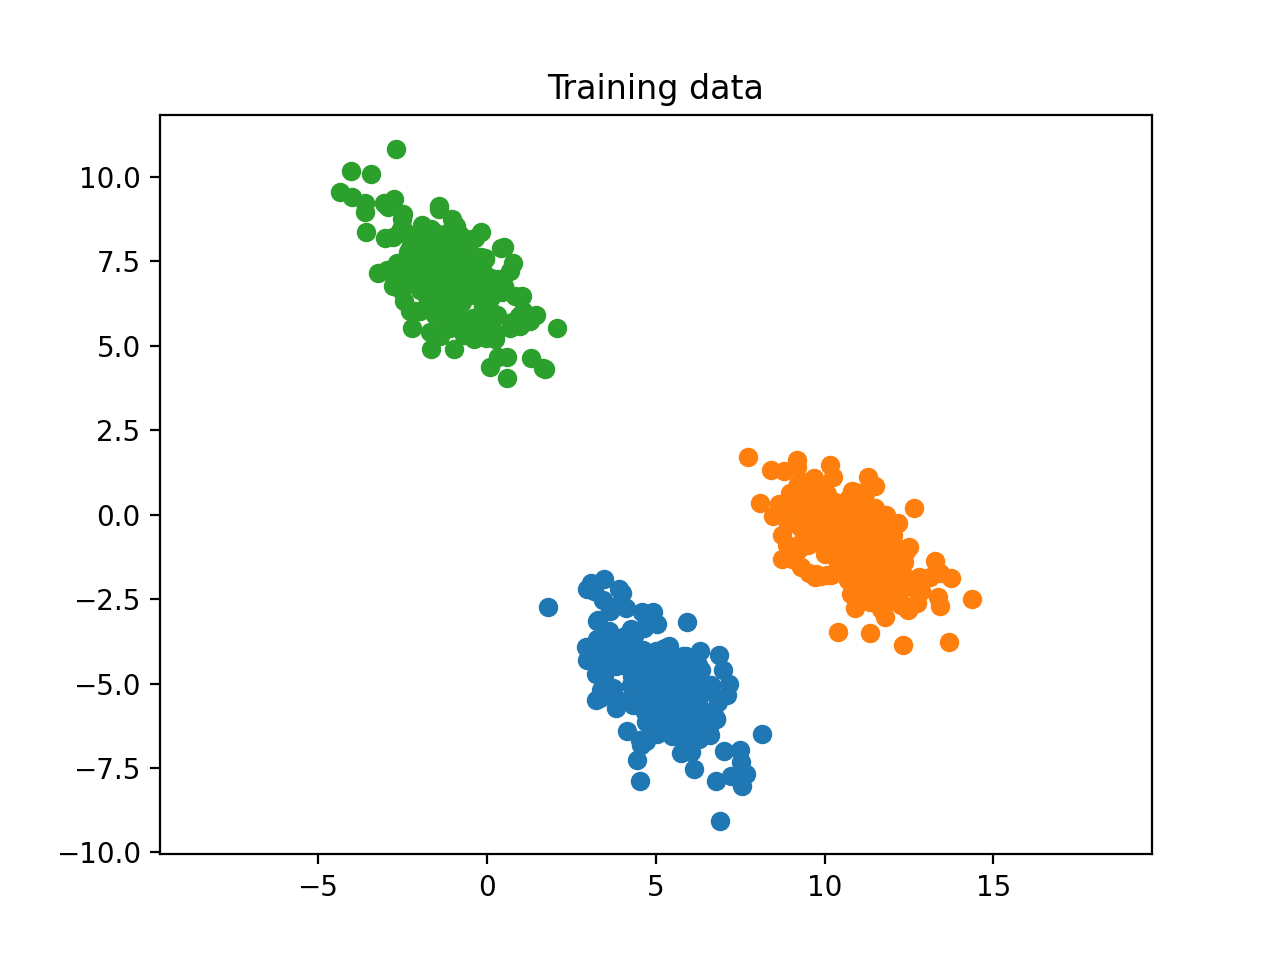
\includegraphics[width=0.48\textwidth]{Figures/LDA_example_original.png}
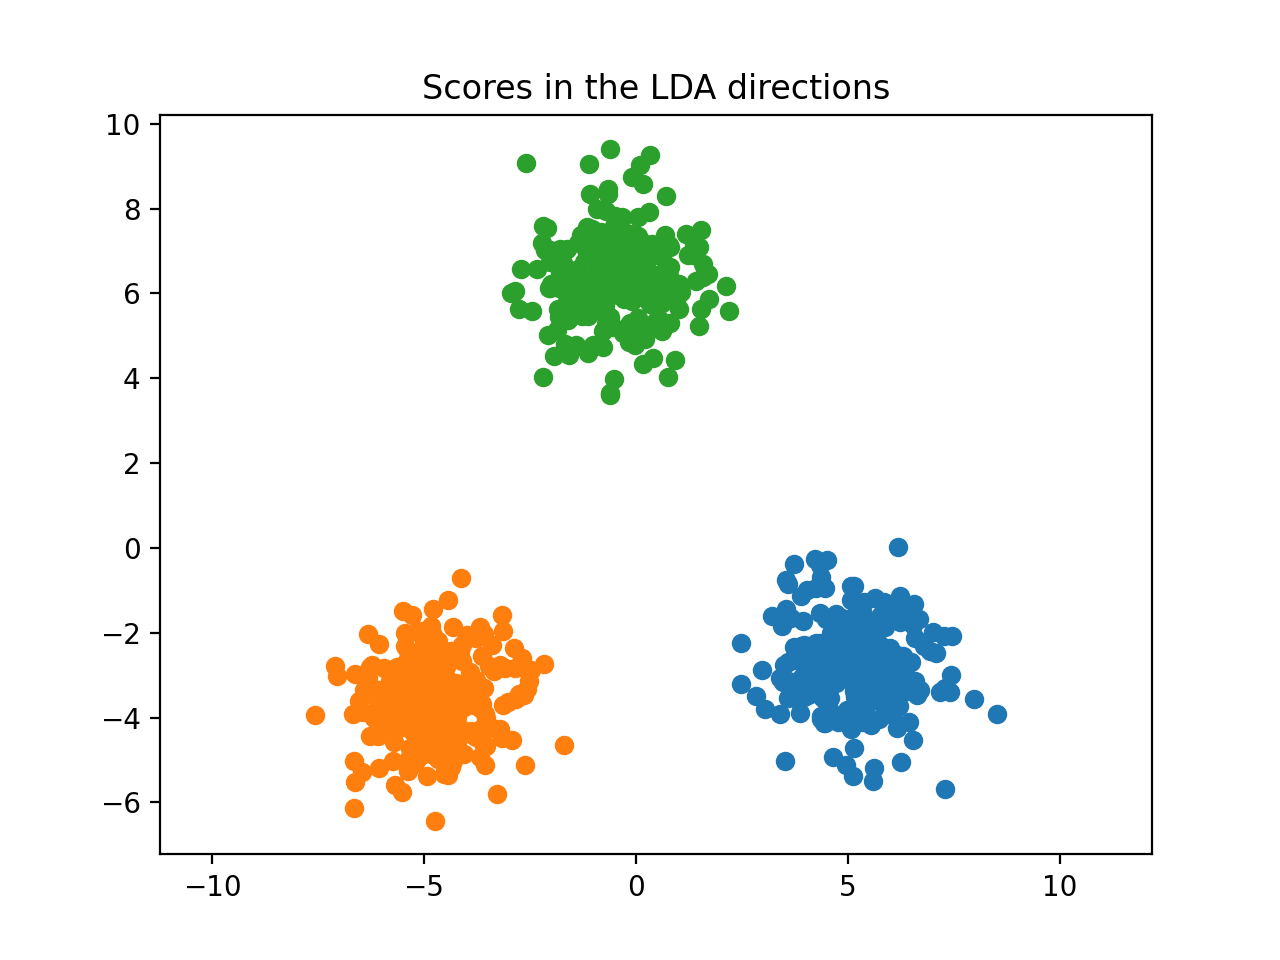
\includegraphics[width=0.48\textwidth]{Figures/LDA_example_scores.png}
\caption{\label{fig:lda} Left: Original (training) data with three classes. Right: LDA scores, where the $x$ axis provides $\ga_1$ and the $y$ axis $\ga_2$.}
\end{figure}



We can now describe the LDA learning algorithm with dimension reduction.
\begin{algorithm}[LDA with dimension reduction]
\begin{enumerate}[label = \arabic*.,wide=0.5cm]
\item Compute $\mu_g, g\in \CR_Y$, $\Sig_w$ and $\Sig_b$ from training data.
\item Estimate (if needed) $\pi_g, g\in \CR_Y$
\item Solve the generalized eigenvalue problem $\Sig_b e = \la\Sig_w e$. Let $e_1, \ldots, e_r$ be the eigenvectors associated with non-zero eigenvalues, normalized so that  $e_j^T \Sig_w e_j = 1$. 
\item Choose a reduced dimension $r_0 \leq r$.
\item Precompute mean scores $\ga_j(\mu_g) = (\mu_g- \mu)^T e_j$, $g\in \CR_Y, j=1, \ldots, r_0$.
\item To classify a new example $x$, compute $\ga_j(x) = (x-\mu)^T e_j$ and choose the class that maximizes 
\[
\sum_{j=1}^{r_0}\ga_j(x)\ga_j(\mu_g) - \frac{1}{2} \sum_{j=1}^{r_0} \ga_j(\mu_g)^2 + \log \pi_g\,.
\]
\end{enumerate}
\end{algorithm}

%Moreover, these $r$ eigenvectors are equivalent to the first $r$ optimal scores defined in section \ref{sec:opt.sc}, through the identity $e_j = \Sig_w^{-1}M\th_j$.

\subsection{Fisher's LDA}
This characterization  leads to the discriminative interpretation of LDA, also called Fisher's LDA. Indeed, the generalized eigenvalue problem $\Sig_b e = \la \Sig_w e$ is directly related to the maximization of the ratio
$e^T\Sig_be$ subject to $e^T\Sig_w e= 1$, which provides directions that have a large between-class variance for within class variance equal to 1. More precisely, $e_1$ is the direction that achieves the maximum; $e_2$ is the second best direction, constrained to being perpendicular to $e_1$, and so on until $e_r$ which is the optimal constrained to be perpendicular to $(e_1, \ldots, e_{r-1})$. We are therefore looking for directions that have the largest ratio of   between-class variance to  within-class variance. 

\subsection{Kernel LDA}

\paragraph{Mean and covariance in feature space}
We assume the usual construction where $h: \CR_X \to H$ is a feature function, $H$ a {Hilbert} space with kernel $K(x,x') = \scp{h(x)}{h(x')}_H$. (The assumption that $H$ is a complete space is here required for the expectations below to be meaningful.)

We now discuss the kernel version of LDA by plugging the feature space representation directly in the classification rule. So, consider $h: \CR \to H$. Let $X:\Om \to \CR$ be a random variable such that $\myE(\|h(X)\|_H^2) < \infty$. Then, its mean feature $m = \myE(h(X))$ is well defined as an element of $H$ , and so are the class averages, $m_g = \myE(h(X)\mid Y=g)$. 

In this possibly infinite-dimensional setting, 
the covariance ``matrix'' is  defined as a linear operator $S: H\to H$ such that, for all $\xi, \eta\in H$:
\begin{equation}
\label{eq:klda.0}
\scp{\xi}{S\eta}_H = \myE\left(\scp{h(X)-m}{\xi}_H\scp{h(X)-m}{\eta}_H\right)\,,
\end{equation}
which is equivalent to defining 
\[
S\eta = E(\scp{h(X)-m}{\eta}_H (h(X) - m))
\] 
for $\eta\in H$.  This definition generalizes the identity for a random variable $U: \Om\to \mR^d$:
\[
S_U w = \myE((U-E(U))(U-E(U))^T) w = \myE(((U-E(U))^Tw)\,(U-E(U))) 
\]
One can similarly define the covariance matrix in class $g$, $S_g$, by conditioning the right-hand side in \cref{eq:klda.0} by $Y=g$ and replacing $m$ by $m_g$. 
\bigskip


\subsubsection*{LDA in feature space}
Following the LDA model, we assume that the operators $S_g$ are all equal to a fixed operator, the within-class  covariance operator denoted $S$.

Assuming that $S$ is invertible, one can generalize the LDA classification rule to data represented in feature space   by classifying a new input $x$ in class $g$ when 
\begin{equation}
\label{eq:klda.1}
\scp{h(x)- m}{ S^{-1} (m_g - m)}_H - \frac12 \scp{m_g - m}{S^{-1} (m_g- m)}_H +  \log\pi_g
\end{equation}
is maximal over all classes. Notice that this is a transcription of the finite-dimensional Bayes rule, but cannot be derived from a generative model, because the assumption that $h(X)$ is Gaussian is not valid in general. (It would require that $h$ takes values in a $d$-dimensional linear space, which would eliminate all interesting kernel representations.)

Let, as before, $T = (x_1, y_1, \ldots, x_N, y_N)$ be the training set,  $N_g$ denote the number of examples in class $g$ and $c_g = N_g/N$.
When $h$ is known (which, we recall, is not a practical assumption, but we will fix this later), one can estimate the class averages from training data by
\[
\mu_g = \frac1{N_g}\sum_{k=1}^N h(x_k) \bfone_{y_k=g}
\]
and the within-class covariance operator by
\[
\scp{\xi}{\Sig_w\eta}_H = \frac1N \sum_{k=1}^N \scp{h(x_k) - \mu_{y_k}}{\xi}_H \scp{h(x_k) - \mu_{y_k}}{\eta}_H.
\]
Unfortunately, the  resulting variance estimator cannot be directly used in \cref{eq:klda.1}, because it is not invertible if $\mathrm{dim}(H) > N$. Indeed, one has $\Sig_w\eta = 0$ as soon as $\eta$ is perpendicular to $V \defeq \vspan(h(x_1), \ldots, h(x_N))$. 

One way to address the degeneracy of the estimated covariance operator is to add to $\Sig_w$ a small multiple of the identity, say $\rho\Id_H$,\footnote{The operator $A + \rho\Id_H$ is invertible as soon as $A$ is symmetric positive semi-definite.} and let the classification rule maximize in $g$:
\begin{multline}
\label{eq:klda.3}
\scp{h(x)-\mu}{ (\Sig_w + \rho\Id_H)^{-1} (\mu_g -  \mu)}_H 
- \frac12 \scp{\mu_g -  \mu}{(\Sig_w + \rho\Id_H)^{-1} (\mu_g-  \mu)}_H + \log\pi_g\,.
\end{multline}
where $\mu$ is the average of $h(x_1), \ldots, h(x_N)$. 
Taking this option, 
we still need to make this expression computable and remove the dependency in the feature function $h$.


\paragraph{Reduction}
We have $\mu_g\in V$ for all $g\in\CR_Y$ and, since 
\[
\Sig_w\eta = \frac1N \sum_{k=1}^N  \scp{h(x_k) - \mu_{y_k}}{\eta}_H (h(x_k) - \mu_{y_k}),
\]
this operator maps $H$ to $V$, which implies that $\Sig_w + \rho \Id_H$ maps $V$ into itself. 
Moreover,  this mapping is onto: If $v\in V$ and $u = (\Sig_w +\rho \Id_H)^{-1}v$, then, $u\in V$.
Indeed, for any $z\perp V$, we have $\scp{z}{\Sig_w u + \rho u}_H = \scp{z}{v}_H$. We have  $\scp{z}{\Sig_w u}_H = 0$ (because $\Sig_w$ maps $H$ to $V$) and $\scp{z}{v}_H = 0$  (because $v\in V$), so that we can conclude that  $\scp{z}{u}_H = 0$. 
 Since this is true for all $z\perp V$, this requires that $u\in V$.\footnote{One has $(V^\perp)^\perp = V$ for finite-dimensional---or more generally closed---subspaces of $H$}

We now express the classification rule in \cref{eq:klda.3} as a function of the kernel associated with the feature-space representation.
Denote, for any vector $u \in \mR^N$, 
\[
\xi(u) = \sum_{k=1}^N \pe u k h(x_k),
\]
 therefore defining a mapping $\xi$ from $\mR^N$ onto $V$. Letting as usual $\CK = \CK(x_1, \ldots, x_N)$ be the matrix formed by pairwise evaluations of $K$ on training inputs, we have the identity
\[
\scp{\xi(u)}{\xi(u')}_H = u^T \CK u'.\
\]
for all $u,u'\in\mR^N$. For simplicity, we will assume in the rest of the discussion that $\CK$ is invertible.

We have $\mu_g = \xi(\dsone_g/N_g)$, where $\dsone_g\in \mR^N$ is the vector with $k$th coordinate equal to 1 if $y_k = g$ and 0 otherwise. Also $\mu = \xi(\dsone/N)$ (recall that $\dsone$ is the vector with all coordinates equal to 1).

For $u\in \mR^N$, we want to characterize $v\in \mR^N$ such that $\Sig_w \xi(u) = \xi(v)$. Let $\de_k$ denote the vector with 1 at the $k$th entry and 0 otherwise. We have
\begin{align*}
\Sig_w \xi(u) &= \frac1N \sum_{k=1}^N  \scp{\xi(u)}{h(x_k) - \mu_{y_k}}_H (h(x_k) - \mu_{y_k})\\
&= \frac1N \sum_{k=1}^N  \scp{\xi(u)}{\xi(\de_k - \dsone_{y_k}/N_{y_k})}_H \xi(\de_k - \dsone_{y_k}/N_{y_k})\\
&= \frac1N \sum_{k=1}^N  ((\de_k - \dsone_{y_k}/N_{y_k})^T \CK u)\, \xi(\de_k - \dsone_{y_k}/N_{y_k})\\
&= \xi\left( \frac1N \sum_{k=1}^N  ((\de_k - \dsone_{y_k}/N_{y_k})^T \CK u)\, (\de_k - \dsone_{y_k}/N_{y_k})\right)
\end{align*}
so that $\Sig_w \xi(u) = \xi(P\CK u)$ with
\[
P = \frac1N \sum_{k=1}^N  (\de_k - \dsone_{y_k}/N_{y_k})(\de_k - \dsone_{y_k}/N_{y_k})^T
\]
Note that one has
\begin{align*}
\bullet\quad & \sum_{k=1}^N  \de_k \de_k^T = \Id[N],\\ 
\bullet\quad&
\sum_{k=1}^N \left(\frac{\dsone_{y_k}}{N_{y_k}}\right) \de_k^T = \sum_{g\in\CR_Y} \frac{\dsone_{g}}{N_{g}} \sum_{k: y_k=g} \de_k^T = \sum_{g\in\CR_Y} \frac{\dsone_{g}\dsone_{g}^T}{N_{g}} = \sum_{k=1}^N \de_k \left(\frac{\dsone_{y_k}}{N_{y_k}}\right)^T,\\
\bullet\quad&
\sum_{k=1}^N \left(\frac{\dsone_{y_k}}{N_{y_k}}\right) \left(\frac{\dsone_{y_k}}{N_{y_k}}\right)^T = \sum_{g\in\CR_Y} \frac{\dsone_{g}\dsone_{g}^T}{N_{g}}.
\end{align*}
This shows that $P$ can be expressed as
\[
P =\frac1N \left( \Id[N] - \sum_{g\in\CR_Y} \dsone_{g}\dsone_{g}^T/N_g\right).
\] 
We have therefore proved that 
\[
\begin{aligned}
\bullet\quad & (\Sig_w + \rho\Id_H) \xi(u) = \xi\left((P\CK + \rho\Id[N]) u\right)\\
\bullet\quad & (\Sig_w + \rho\Id_H)^{-1} \xi(\tilde u) = \xi\left((P\CK + \rho\Id[N])^{-1} \tilde u \right).
\end{aligned}
\]
 Recall that the feature-space LDA classification rule maximizes
\[
\scp{h(x)-\mu}{ (\Sig_w + \rho\Id_H)^{-1} (\mu_g -  \mu)}_H 
- \frac12 \scp{\mu_g -  \mu}{(\Sig_w + \rho\Id_H)^{-1} (\mu_g-  \mu)}_H + \log\pi_g\,.
\]
 All terms belong to $V$, except $h(x)$, but this term can be replaced by its orthogonal projection on $V$ without changing the result. This projection can be made explicit in terms of the representation $\xi$ as follows. 
For $x\in \CR$, let $\xi(\psi(x))$ denote the orthogonal projection of $h(x)$ on $V$ (this defines the function $\psi$). If $v(x)$ denotes the vector with coordinates $K(x, x_k)$, $k=1, \ldots, N$, then $\psi(x) = \CK^{-1} v(x)$, as can be obtained by identifying the inner products $\scp{h(x)}{h(x_k)}_H$ and $\scp{\xi(\psi(x))}{h(x_k)}_H$.

We are now ready to rewrite the kernel LDA classification rule in terms of quantities that only involve $K$. We have  
\[
\begin{aligned}
&\scp{h(x)-\mu}{ (\Sig_w + \rho\Id_H)^{-1} (\mu_g - \mu)}_H \\
 & = \scp{\xi(\psi(x) - \dsone/N)}{\xi((P\CK + \rho\Id[N])^{-1} (\dsone_g/N_g - \dsone/N))}_H\\
&= (\psi(x) - \dsone/N)^T\CK(P\CK + \rho\Id[N])^{-1} (\dsone_g/N_g - \dsone/N)
\end{aligned}
\]
 Given this, the classification rule must maximize
\begin{multline}
(\psi(x) - \dsone/N)^T\CK (P\CK + \rho\Id[N])^{-1} (\dsone_g/N_g - \dsone/N)\\
 - \frac12 (\dsone_g/N_g - \dsone/N)^T \CK (P\CK + \rho\Id[N])^{-1} (\dsone_g/N_g - \dsone/N) + \log\pi_g.
\label{eq:klda.V}
\end{multline}

\paragraph{Dimension reduction}
Note that $\CK (P\CK + \rho\Id[N])^{-1} = \CK (\CK P\CK + \rho\CK)^{-1} \CK$ is a symmetric matrix. So, the expression in \cref{eq:klda.V} can be written as
\[
(v(x) - \nu )^T R^{-1} (\nu_g - \nu)
 - \frac12 (\nu_g - \nu)^T R^{-1} (\nu_g - \nu) + \log\pi_g.
\]
with $R = \CK P\CK + \rho\CK$, $\nu_g = \CK \dsone_g/N_g$ and $\bar\nu = \CK \dsone /N$. Clearly, if $v_1, \ldots, v_N$ are the column vectors $\CK$, we have
\[
\nu_g = \frac1{N_g} \sum_{k=1}^N v_k \bfone_{y_k=g},
\quad
\bar\nu = \frac1N \sum_{k=1}^N v_k\,.
\]


We therefore retrieve an expression similar to  finite-dimensional LDA, provided that one replaces $x$ by $v(x)$, $x_k$ by $v_k$ and $\Sig_w$ by  $R$. Letting 
\[
Q= \frac1N \sum_{g\in \CR_Y} N_g (\nu_g-\bar\nu)(\nu_g-\bar\nu)^T
\]
be the between-class covariance matrix, 
the discriminant directions are therefore  solutions of the generalized eigenvalue problem
\[
Q f_j = \la_j R f_j
\]
with $f_j^TRf_j = 1$ with $R=(\CK P\CK + \rho \CK)$. Note that 
\[
\CK P \CK = \frac1N \sum_{k=1}^N (v_k - \bar\nu_{y_k})(v_k - \bar\nu_{y_k})^T
\]
is the within-class covariance matrix for the training data $(v_1, y_1, \ldots, v_N, y_N)$.

The following summarizes the kernel LDA classification algorithm.
\begin{algorithm}[Kernel LDA]
\label{alg:k.lda}
\begin{enumerate}[label=(\arabic*)]
\item Select a positive kernel $K$ and a coefficient $\rho >0$.
\item Given $T = (x_1, y_1, \ldots, x_N, y_N)$ and a kernel $K$, compute the kernel matrix $\CK = \CK(x_1, \ldots, x_N)$ and the matrix $R = \CK P\CK + \rho \CK$. Let $v_1, \ldots, v_N$ be the column vectors of $\CK$.
\item Compute, for $g\in \CR_Y$, 
\[
\nu_g = \frac1{N_g} \sum_{k=1}^N v_k \bfone_{y_k=g}\, ,
\quad
\bar\nu = \frac1N \sum_{k=1}^N v_k
\]
and let $Q = \frac1N \sum_{g\in \CR_Y} N_g (\nu_g-\bar\nu)(\nu_g-\bar\nu)^T$.
\item Fix $r_0 \leq q-1$ and compute the eigenvectors $f_1, \ldots, f_{r_0}$ associated with the $r_0$ largest eigenvalues for the generalized eigenvalue problem $Qf = \la Rf$, normalized such that $f_j^T R f_j = 1$.
\item Compute the scores $\ga_{jg} = (\nu_g-\bar\nu)^Tf_j$.
\item Given a new observation $x$, let $v(x)$ be the vector with coordinates $K(x,x_k)$, $k=1, \ldots, N$. Compute the scores $\ga_j(x) = (v(x) - \bar\nu)^T f_j$, $j=1, \ldots, r_0$. Classify $x$ in the class $g$ maximizing 
\begin{equation}
\label{eq:klda.final}
\sum_{i=1}^r \ga_i(x) \ga_{ig} - \frac12 \sum_{i=1}^r \ga_{ig}^2  + \log\pi_g.
\end{equation}
\end{enumerate}
\end{algorithm}



%Introduce the solutions of the generalized eigenvalue problem
%\[
%\CK P \CK e_i = \la_i \CK e_i
%\]
%for $i=1, \ldots, N$, normalized so that $e_i^T\CK e_i = \|\xi(e_i)\|^2_H = 1$. This is equivalent to letting $Se_1, \ldots Se_N$ be an orthonormal basis of eigenvectors of $SPS$, with $\S = \CK^{1/2}$.  In particular, for any vector $a\in \mR^N$, one has
%\begin{multline*}
%(P\CK + \rho \Id)^{-1} a = S^{-1}(SPS +\rho\Id) Sa \\ = \sum_{i=1}^N \frac{(Sa)^T(Se_i)}{\la_i + \rho} S^{-1}(Se_i)
%=  \sum_{i=1}^N \frac{e_i^T \CK a}{\la_i + \rho} e_i\,.
%\end{multline*}
%This implies that, for any $a, a'\in \mR^N$,
%\begin{multline*}
%\scp{\xi(a')}{\xi((P\CK + \rho \Id)^{-1} a)}_H \\ = \sum_{i=1}^N \frac{e_i^T \CK a}{\la_i + \rho} \scp{\xi(a')}{\xi(e_i)}_H 
%= \sum_{i=1}^N \frac{(e_i^T \CK a)(e_i^T\CK a')}{\la_i + \rho}\,.
%\end{multline*}  
%We can now make explicit the classification rule in \eqref{eq:klda}, with $S_w$ replaced by $\Sig_w + \rho\Id$. We have , so that 
%\begin{align*}
%\scp{\mu_g - \bar\mu}{(\Sig_w + \rho\Id)^{-1} (\mu_g - \bar \mu)}_H &= \sum_{i=1}^N \frac{(e_i^T \CK a_g)^2}{\la_i + \rho}
%\end{align*}
%with $a_g = \bfone_g/N_g - \bfone/N$. Similarly 
%\begin{align*}
%\scp{h(x) - \bar\mu}{(\Sig_w + \rho\Id)^{-1} (\mu_g - \bar \mu)}_H &= 
%\sum_{i=1}^N \frac{e_i^T \CK a_g}{\la_i + \rho} \scp{h(x) - \bar\mu}{\xi(e_i)}_H
%\end{align*}
%with
%\[
%\scp{h(x) - \bar\mu}{\xi(e_i)}_H = \ka(x)^Te_i - \frac{1}{N} \bfone^T\CK e_i
%\]
%where $\ka(x)$ is the vector with coordinates $K(x, x_k)$, $k=1, \ldots, N$. 
%
% where
%$$
%\Sig_w = \frac{1}{N} \sum_{k=1}^N (h_(x_k) -
%\bar\mu_{y_k})(h(x_k) - \bar\mu_{y_k})^T
%$$
%is the within-class covariance matrix, $\mu_g$ are class averages (of features) and $\bar\mu$ the global average. 
%In infinite-dimensional feature spaces, however, the ``matrix'' $\Sig_w$ cannot
%be invertible. Indeed, as soon as a vector $v$ is orthogonal to all
%the $h_k - \bar\mu$ (and hence to all the $\mu_g-\bar\mu$), we have
%$$
%\Sig_w v = \frac{1}{N} \sum_{k=1}^N (h_k -
%\bar\mu_{y_k})\scp{h_k - \bar\mu_{y_k}}{v}_H = 0.
%$$
%Therefore, LDA cannot be directly generalized to the infinite-dimensional setting.
%
%This issue can be bypassed by restricting to the affine space $H_0 = \bar\mu +
%\text{span}(h_k-\bar\mu, k=1, \ldots, N)$. Centering by $\bar\mu$ in
%feature space is then equivalent to using the ``centered kernel''
%\begin{eqnarray*}
%\bar K(x,y) &=& \scp{h(x)- \bar\mu}{h(y)- \bar\mu}_H\\
%&=& K(x,y) - \frac{1}{N} \sum_{k=1}^N (K(x_k,y) + K(x_k,x))
%+ \frac{1}{N^2} \sum_{k,l=1}^N K(x_k,x_l).
%\end{eqnarray*}
%It is easy to check that replacing $K$ by $\bar K$ is equivalent to
%assuming $\bar\mu=0$. This will lighten the formulas in the following computations.
%We also define
%$$
%r_g(x) = \scp{h(x)}{\mu_g} = \frac{1}{N_g} \sum_{k=1}^N \bar K(x, x_k)
%\chi_{y_k=g}.
%$$ 
%
%It will be more convenient to work with Fisher's formulation of
%discriminant analysis, which consists in maximizing the ratio
%$$
%\frac{v^T\Sig_b v}{v^T \Sig_w v}.
%$$
%Taking
%$v$ in the form
%$$
%v = \sum_{k=1}^N  \al_k  h_k,
%$$
%we now express the maximization problem in terms of $\al$. We have
%\begin{eqnarray*}
%v^T\Sig_b v &=& \sum_{g\in \CR_Y} N_g (v^T \mu_g )^2\\
%&=& \sum_{g\in\CR_Y} N_g\left(\sum_{k=1}^N \al_k r_{g}(x_k) \right)^2\\
%&=& \sum_{k,l=1}^N \al_k\al_l \sum_{g\in \CR_Y} N_g r_g(x_k) r_g(x_l) \\
%&=& \al^T Q \al
%\end{eqnarray*}
%where $Q$ is the  matrix with coefficients $q_{kl}  =
%\sum_{g\in \CR_Y} N_g r_g(x_k) r_g(x_l)$.
%
%Letting $\Sig$ be the global covariance matrix (so that $\Sig_w =
%\Sig-\Sig_b$), we have
%\begin{eqnarray*}
%v^T\Sig v &=& \sum_{k=1}^N (v^T h_k )^2\\
%&=& \sum_{k=1}^N N_g \left(\sum_{l=1}^N \al_k \bar K(x_k,x_l) \right)^2\\
%&=& \sum_{k,l=1}^N \al_k\al_l \sum_{l'=1}^N  \bar K(x_k,x_{l'})\bar K(x_{l'},x_l) \\
%&=& \al^T S \al
%\end{eqnarray*}
%with $s_{kl} = \sum_{l'=1}^N  \bar K(x_k,x_{l'})\bar K(x_{l'},x_l)$.
%
%The ratio of variances is therefore given by $\al^T Q \al / \al^T
%(S-Q)\al$. The optimal $\al$ is given by the first eigenvector of
%$(S-Q)^{-1}Q$, the following eigenvectors providing subsequent
%discriminant directions. 
%
%
%At a result of this procedure, we get a family of directions, $v_1,
%\ldots, v_q$ in feature space, with coefficients $\al_1, \dots, \al_q$
%such that
%$$
%v_j = \sum_{k=1}^N \al_{jk} h_k,\   j=1, \ldots, q.
%$$
%As remarked in section \ref{sec:lda}, the squared distance (for
%$\Sig_w^{-1}$) between $h(x)$ and a class 
%average $\mu_g$ is directly given (after projection on
%$\text{vect}(v_1, \ldots, v_q)$ by
%$$
%\sum_{j=1}^q (\scp{h(x)}{v_j}_H - \scp{\mu_g}{v_j}_K)^2.
%$$
%These dot products are directly computed from the $\al$'s and the
%centered kernel, as
%$$
%\scp{h(x)}{v_j}_H = \sum_{k=1}^N \al_{jk} \bar K(x, x_k) \text{ and }
%\scp{\mu_g}{v_j}_H = \sum_{k=1}^N \al_{jk}  r_g(x_k).
%$$
%


%Since $(\tilde e_1, \ldots, \tilde e_r) \in V$, they can be written as linear combinations
%of the $\tilde\mu_g$'s, so there there must exist a $q$ by $r$
%matrix $\tilde A$ such that
%$$
%\tilde E: = [\tilde e_1, \ldots, \tilde e_{r}] = \tilde M \tilde A.
%$$
%To have an orthonormal
%family, we need $\tilde E^T\tilde E = \Id_{r}$ yielding
%$$
%\Id_{r} = \tilde A^T  \tilde M^T \tilde M \tilde A.
%$$
%The matrix $\tilde M^T\tilde M$ is the Gram matrix of $\tilde\mu_1, \ldots, \tilde\mu_q$, a $q$ by $q$ matrix formed
%with the dot products of the $\tilde \mu_g$'s. Its rank is the dimension of
%$V$. Let $\tilde a_1, \ldots, \tilde a_q$ form an orthonormal basis of  eigenvectors of $\tilde M^T \tilde M$, 
%associated to decreasing eigenvalues $\la_1, \ldots, \la_q$ (the first
%$r$ being non-vanishing, the last $q-r$ being 0). Then, it is an easy computation to check
%that 
%$\tilde A_0 = [\tilde a_1/\sqrt{\la_1},
%\ldots, \tilde a_{r}/\sqrt{\la_r}]$ satisfies the required
%identity. Moreover, any other solution must correspond to a change of orthonormal family in $V$ and therefore take the form $\tilde A = \tilde A_0 R$ where $R$ is an $r$ by $r$ orthogonal matrix. 

%This is not the only solution that we can get this way,
%however. In fact, if $S$ is any invertible $q$ by $q$
%matrix, we can apply the same computation replacing $\tilde A$ by
%$S\tilde A$,
%yielding
%$$
%\Id_{r} = \tilde A^T S^T  \tilde M^T \tilde M S \tilde A,
%$$
%and let $\tilde a_1, \ldots, \tilde a_q$ be the eigenvectors of
%$S^T \tilde M^T \tilde M S$, still taking 
%$\tilde A = [\tilde a_1/\sqrt{\la_1},
%\ldots, \tilde a_{r}/\sqrt{\la_r}]$ for the corresponding eigenvalues. We will assume that such an $S$ is
%chosen in the rest of the computation.
%



%These scores have a nice expression in terms of the original
%variables. Using the fact that $\tilde M^T \tilde
%M = M^T \Sig_w^{-1} M$, we have, from the definition of $\tilde $A_0$
%\begin{equation}
%\label{eq:lda.1} 
%M^T \Sig_w^{-1} M \tilde A_0= \tilde A_0 \La. 
%\end{equation}
%
%
% By construction
%$S^T\tilde M^T\tilde M S\tilde A = \tilde A \La$, where $\La =
%\mathit{diag}(\la_1, \ldots, \la_r)$,  yielding
%\begin{equation}
%\label{eq:lda.1} 
%S^TM^T \Sig_w^{-1} MS \tilde A= \tilde A \La. 
%\end{equation}
%We also have  $\tilde MS\tilde A = \tilde E$, yielding
%$\Sig_w^{-1/2} MS\tilde A = \tilde E$; multiplying both sides in
%\eqref{eq:lda.1} by $\Sig_w^{-1/2}MS$ we get
%$$
%\Sig_w^{-1/2} MSS^TM^T \Sig_w^{-1/2} \tilde E = \tilde E \La.
%$$ 
%Multiplying the result by $\Sig_w^{-1/2}$ and letting $ E =
%\Sig_w^{-1/2} \tilde E$, we finally get
%$$
%\Sig_w^{-1} MSS^TM^T E = E \La
%$$
%so that $E$ is a matrix formed with the eigenvectors of $\Sig_w^{-1}
%MSS^TM^T $ (but normalized so that $E^T\Sig_w^{-1} E = \Id_r$).
%These properties permit to compute $E$, from which all scores can be
%computed since
%$$
%\ga_j(x) = x^T \Sig_w^{-1/2} \tilde e_j = x^T e_j.
%$$
%Letting $Q = SS^T$ (any positive definite matrix can take this form)
%and 
%$$
%\Sig_b^Q = MQM^T = \sum_{g\in\CR_Y} q_{gh} (\mu_g-\mu) (\mu_h-\mu)^T, 
%$$
%we see that $e_1, \ldots, e_r$ are eigenvectors of of $\Sig_w^{-1}
%\Sig_b^Q$, so that, for some $\la_j$:
%$$
%\Sig_b^Q e_j = \Sig_w e_j.
%$$
%This is the generalized eigenvalue problem associated to $\Sig_b^Q$
%and $\Sig_w$. The first eigenvector is the maximizer of the ratio
%$$
%u\mapsto \frac{u^T\Sig_b^Q u}{u^T\Sig_w u}
%$$
%and the following ones maximize this ratio subject to the constraint of
%being perpendicular to those that precede. With $Q =
%\mathit{diag}(c_{g_1}, \ldots, c_{g_q})$, we have
%$$
%\Sig_b^Q = \Sig_b := MCM^T  = \sum_{g\in \CR_Y} c_g (\mu_g-\mu)
%(\mu_g-\mu)^T
%$$
%which is called the between class (or interclass) covariance
%matrix. The method or progressively maximizing the ratio 
%${u^T\Sig_b^Q u}/{u^T\Sig_w u}$ is called {\em Fisher's linear
%  discriminant analysis}. 
%
%\section{Optimal scoring}
%



\section{Optimal Scoring}
\label{sec:opt.sc}

It is possible to apply linear regression (\cref{chap:lin.reg}) to solve a classification problem by mapping  the set $\CR_Y$ to a collection of $r$-dimensional row vectors, or ``scores.''  These scores (which have a different meaning from the LDA scores) will be represented by a function $\th : \CR_Y \mapsto \mR^r$. As an example, one can  take $r=q$ and 
\[
\th(g_1) = \begin{pmatrix} 1\\ 0\\0\\ \vdots\\0\end{pmatrix},\ 
\th(g_2) = \begin{pmatrix} 0\\ 1\\0\\ \vdots\\0\end{pmatrix},\,\ldots\,, \ 
\th(g_q) = \begin{pmatrix} 0\\ 0\\ \vdots\\0\\1\end{pmatrix}.
\]
Given a training set $T = (x_1, y_1, \ldots, x_N, y_N)$ and a score function $\th$, a linear
model can then be estimated from  data by minimizing
$$
\sum_{k=1}^N |\th_{y_k} - {a_0} - b^T  x_k|^2
$$ 
where $b$ is a $d \ti
q$ matrix and ${a_0} \in \mR^q$. Letting as before $\be$ be the matrix with $a_0^T$ added as first row to $b$ and $\CX$ the matrix with first row containing only ones and subsequent rows given by $x_1^T, \ldots, x_N^T$, one gets the least square estimator
$\hat \beta = (\CX^T\CX)^{-1}\CX^T\CY$, where $\CY$ is the $N\times q$
matrix of stacked $\th^T_{y_k}$ row vectors. 

Given an input vector $x$, the row vector $\tilde x^T\beta$ will generally not coincide with one of the score vectors.  Assignment to a class can   then be
made by minimizing $|{a_0} + b^T x - \th_{g}|$ over all
$g$ in $\CR_Y$.\bigskip


Since the scores $\th$ are free to choose, one may also try to optimize them, resulting in the \alert{optimal scoring} algorithm. To describe it, we will need the notation already introduced for LDA, plus the following.  We will write, for short,  $\th_j = \th(g_j)$ and introduce the $q\times r$ matrix $\Th = \begin{pmatrix} \th_1^T\\ \vdots\\ \th_q^T\end{pmatrix}$.
We also denote by  $\rho_1, \ldots, \rho_r$ the column vectors of $\Th$, so that $\Th = [\rho_1, \ldots, \rho_r]$. 
Let $u_{g_i}$, for $i=1, \ldots, q$, denote the $q$-dimensional vector with $i$th coordinate equal to 1 and all others equal to 0.
As before, $N_g$ denote the class sizes,  $c_g = N_g/N$, $C$ is the diagonal matrix with coefficients $c_{g_1}, \ldots, c_{g_q}$ and $\ze = \begin{pmatrix} c_{g_1}\\ \vdots \\c_{g_q}\end{pmatrix}$.

The goal of optimal scoring is to minimize, now with respect to $\th$, ${a_0}$ and $b$, the function
\[
F(\th, {a_0}, b) = \sum_{k=1}^N |\th(y_k) - {a_0} - b^T  x_k|^2\,.
\]
Some normalizing conditions are clearly needed, because this problem is under-constrained. (In the  form above, the optimal choice is to take all free parameters equal to 0.) We now discuss the various indeterminacies and redundancies in the model, 

\begin{enumerate}[label = (\alph*), wide=0cm]
\item If $R$ is an $r\times r$ orthogonal matrix, then $F(R\th, R{a_0}, bR^T) = F(\th, {a_0}, b)$, yielding an infinity of possible equivalent solutions (that all lead to the same classification rule).
This implies that there is no loss of generality in assuming that $\Th^T C \Th$ is diagonal (introducing $C$ here will turn out to be convenient). Indeed, given any $(\th, {a_0}, b)$, one can just take $R$ such that $R\Th^T C \Th R^T$ is diagonal and replace $\Th$ by $R\Th$, ${a_0}$ by $R{a_0}$ and $b$ by $bR^T$ to get an equivalent solution satisfying the constraint.
\item Let $D$ be an $r$ by $r$ diagonal matrix with positive entries. Replace $\th$, ${a_0}$ and $b$ respectively by $D\th$, $D{a_0}$ and $bD$. The resulting objective function is 
\[
\begin{aligned}
F(D\th, D{a_0}, bD^T) &= \sum_{k=1}^N |D\th(y_k) - D{a_0} - Db^T  x_k|^2 \\
&= \sum_{j=1}^r \sum_{k=1}^N d_{jj}^2 \Big(\th(y_k, j) - {a_0}(j) - \sum_{i=1}^d b(i,j)  x_k(i)\Big)^2
\end{aligned}
\]
If the coefficient $d_{jj}$ is free to chose, then the objective function can always be reduced by letting $d_{jj} \to 0$, which removes one of the dimensions in $\th$. In order to avoid this, one needs to  fix the diagonal values of  $\Th^T C\Th$, and, by symmetry, it is natural to require  $\Th^T C\Th = \Id[r]$. 
\item Given any $\delta\in \mR^r$, one has $F(\th, {a_0}, b) = F(\th-\de, {a_0}+\de, b)$, with identical classification rule.
One can therefore without loss of generality introduce $r$ linear constraints, and a convenient choice is 
\[
\Th^T\ze = \sum_{g\in \CR_Y} c_g\th_g= 0.
\]
\end{enumerate}
\medskip

Given this reduction, we can now describe the optimal scoring problem as the minimization of 
\[
\sum_{k=1}^N |\th_{y_k} - {a_0} - b^T x_k|^2
\]
subject to $\Th^TC\Th = \Id[r]$ and $\Th^T\ze = 0$. 

The optimal ${a_0}$ is given by
\[
\hat{a_0} = \frac1N \sum_{k=1}^N \th_{y_k} - b^T\mu = -b^T\mu,
\]
so that the problem is reduced to minimizing 
\[
\sum_{k=1}^N |\th_{y_k} - b^T (x_k-\mu)|^2
\]
subject to the same constraints. Using the facts that $\th_{y_k} = \Th^T u_{y_k}$, that
\[
\sum_{k=1}^N u_{y_k}u_{y_k}^T = \sum_{g\in \CR_Y} N_g u_{g}u_{g}^T = NC
\]
and that
\begin{align*}
\sum_{k=1}^N u_{y_k}(x_k-\mu)^T &= \sum_{g\in \CR_Y}^N u_{g} \sum_{k: y_k = g} (x_k-\mu)^T
= \sum_{g\in \CR_Y}^N u_{g} N_g (\mu_g - \mu)^T = NCM,
\end{align*}
one can write 
\[
\begin{aligned}
\sum_{k=1}^N |\th_{y_k} - b^T (x_k-\mu)|^2 &= \sum_{k=1}^N |\Th^T u_{y_k} - b^T (x_k-\mu)|^2 \\
&= \sum_{k=1}^N u_{y_k}^T \Th \Th^T u_{y_k} - 2 \sum_{k=1}^N (x_k-\mu)^T b\Th^Tu_{y_k} + \sum_{k=1}^N (x_k-\mu)^T bb^T (x_k-\mu)\\
&= \sum_{k=1}^N \trace(\Th^T u_{y_k}u_{y_k}^T \Th) - 2 \sum_{k=1}^N \trace(\Th^T u_{y_k} (x_k-\mu)^T b) \\
& \qquad + \sum_{k=1}^N \trace( b^T (x_k-\mu)(x_k-\mu)^T b)\\
&= N\trace(\Th^TC\Th) - 2N\trace(\Th^TCMb) + N\trace(b^T\Sig_{XX}b)\,.
\end{aligned}
\]

Note that, since $\Th^T C \Th= \Id[r]$, then $\trace(\Th^TC\Th)=r$. 
We therefore obtain a concise form of the optimal scoring problem: minimize
\[
- 2\trace(\Th^TCMb) + \trace(b^T\Sig_{XX}b).
\]
subject to $\Th^T C \Th= \Id[r]$ and $\Th^T\ze = 0$.

Given $\Th$,  the optimal $b$ is  $\Sig_{XX}^{-1} M^TC\Th$, and replacing it in the objective function, one finds that $\Th$ must minimize
\[
- 2\trace(\Th^TCM\Sig_{XX}^{-1} M^TC\Th) + \trace(\Th^TCM\Sig_{XX}^{-1} M^TC\Th)
\]
i.e., maximize
\[
\trace(\Th^T CM\Sig_{XX}^{-1} M^T C \Th)
\]
subject to $\Th^T C \Th= \Id[r]$ and $\Th^T\ze = 0$.  We now recall the following linear algebra result (see \cref{chap:linalg}). 
\begin{proposition}
\label{prop:gen.eig}
Let $A$ and $B$ be respectively positive definite and non-negative semi-definite symmetric $q$ by $q$ matrices. Then, the maximum, over all $q$ by $r$ matrices $S$ such that $\trace(S^TAS) = \Id[r]$, of $\trace(S^TBS)$   is attained at $S = [\sig_1, \ldots, \sig_r]$, where the columns vectors $\sig_1, \ldots, \sig_r$ are the solutions of the generalized eigenvalue problem
\[
B\sig = \la A\sig
\]
associated with the largest eigenvalues, normalized so that $\sig_i^T A \sig_i = 1$ for $i=1, \ldots, r$..
\end{proposition}

Given this proposition, let $\rho_1, \ldots, \rho_r$ be the $r$ first  eigenvectors for the problem
\begin{equation}
\label{eq:ge.os}
CM\Sig_{XX}^{-1} M^T C\rho = \lambda C\rho.
\end{equation}
Assume that $r$ is small enough so that the associated eigenvalues are not zero.
Let  $\Th = [\rho_1, \ldots, \rho_r]$. We now prove that $\Th$ is indeed a solution of the optimal scoring problem, and the only point to show to complete the statement is that this $\Th$ satisfies the constraints  $\Th^T\ze = 0$.
 But we have
\[
M^TC\dsone_q = \sum_{g} c_g (\mu_g - \bar\mu) = 0, 
\]
which implies that $\dsone_q$ is a solution of the generalized eigenvalue problem associated with $\la = 0$. This in turn implies that $\dsone_q^T C \rho_i  = \ze^T \rho_i=  0$, which is exactly $\Th^T\ze  = 0$.  
\bigskip

To summarize, we have  found that the solution $\th, b$ minimizing 
\[
- 2\trace(\Th^TCMb) + \trace(b^T\Sig_{XX}b)
\]
subject to $\Th^T C \Th= \Id[r]$ and $\Th^T\ze = 0$ is given by
\begin{enumerate}[label=(\roman*)]
\item $\Th = [\rho_1, \ldots, \rho_r]$ where $\rho_1, \ldots, \rho_r$ are the eigenvectors for the problem
\[
CM\Sig_{XX}^{-1} M^T C\rho = \lambda C\rho
\]
associated with the $r$ largest eigenvalues, normalized so that $\rho^TC\rho = 1$. 
\item $b = \Sig_{XX}^{-1} M^TC\Th$.
\end{enumerate}

The computation can, however, be further simplified.
Let $\la_1, \ldots, \la_r$ be the eigenvalues associated with $\rho_1, \ldots, \rho_r$. Letting $D$ be the associated diagonal matrix, one can write
\[
CM\Sig_{XX}^{-1} M^T C\Th = C\Th D.
\]
This yields
\[
\Th = M\Sig_{XX}^{-1} M^T C\Th D^{-1} = MbD^{-1},
\]
from which we deduce that $\th_g = \Th^T u_g = D^{-1} b^T(\mu_g - \bar\mu)$. So, given a new input vector $x$, the decision rule is to assign it to the class $g$ for which 
\[
|\th_g - b^T(x-\bar\mu)|^2 =  |\Th^T u_g - b^T(x-\bar\mu)|^2 = |D^{-1} b^T(\mu_g - \bar\mu) - b^T(x-\bar\mu)|^2
\]
is minimal. Letting $b_1, \ldots, b_r$ denote the $r$ columns of $b$, this is equivalent to minimizing, in $g$
\begin{equation}
\label{eq:os.rule}
\sum_{j=1}^r (b_j^T (\mu_g - \bar\mu))^2/\la_j^2 - 2 \sum_{j=1}^r (b_j^T (x - \bar\mu))(b_j^T (\mu_g - \bar\mu))/\la_j.
\end{equation}

From $b = \Sig_{XX}^{-1} M^T C \Th$ and $\Th = MbD^{-1}$ we see that 
\[
bD = \Sig_{XX}^{-1} M^T C Mb ,
\]
so that $ \Sig_b b = \Sig_{XX} b D$.
This shows that the columns of $b$ are solution of the eigenvalue problem $\Sig_b u = \la \Sig_{XX} u$. 
Moreover, from $\Th^T C \Th = \Id[r]$, we get $b^T \Sig_b b = D^{2}$. 
Since $b^T   \Sig_b b = b^T\Sig_{XX} b D$, we get that $b$ must be normalized to that $b^T\Sig_{XX} b = D$. 

This shows that the solution of the optimal scoring problem can be reformulated uniquely in terms of $b$: 
if $b_1, \ldots, b_r$ are the $r$ principal solutions of the eigenvalue problem  $\Sig_b u = \la \Sig_{XX} u$, normalized so that $u^T \Sig_{XX} u = \la$, a new input is classified into the class $g$ minimizing
\[
\sum_{j=1}^r \ga_j(\mu_g)^2/\la_j^2 - 2 \sum_{j=1}^r \ga_j(x) \ga_j(\mu_g) /\la_j.
\]
with $\ga_j(x) = b_j^T (x - \bar\mu)$. 




\bigskip

\begin{remark}
The following computation shows that optimal scoring is closely related to LDA. 
 Recall the identity $\Sig_{XX} = \Sig_w + \Sig_b$.
It implies that a solution of $\Sig_b u = \la \Sig_{XX} u$ is also a solution of $\Sig_b u = \tilde \la \Sig_{w} u$ with $\tilde \la = \la/(1-\la)$. 
If  $u^T \Sig_{XX} u = \la$, then 
\[
 u^T \Sig_{w} u = \la - u^T \Sig_{b} u = \la - \la^2 = \frac{\tilde \la}{(1+\tilde \la)^2},
 \]
which shows that 
 \[
 \tilde u = \frac{1+\tilde \la}{\sqrt{\tilde\la}} u
 \]
 satisfies $\tilde u^T \Sig_{w} \tilde u = 1$. 
So, 
 \[
 e_j = \frac{1+\tilde \la_j}{\sqrt{\tilde\la_j}} b_j
 \]
 coincide with the LDA directions.
  We have, letting $\tilde \ga_j(x) = e_j^T (x - \bar\mu) = \sqrt{\tilde\la_j}\ga_j(x)/(1+\tilde \la_j)$:
\begin{multline*}
\sum_{j=1}^r \ga_j(\mu_g)^2/\la_j^2 - 2 \sum_{j=1}^r \ga_j(x) \ga_j(\mu_g) /\la_j = 
\sum_{j=1}^r \tilde \ga_j(\mu_g)^2/\tilde \la_j  - 2\sum_{j=1}^r \ga_j(x) \ga_j(\mu_g)/ (1+\tilde \la_j) 
\end{multline*}
which relates the classification rules for the two methods.
\end{remark}

% the optimal scores directly provide the
%first discriminant direction. More precisely, if $e_1$ is, as above,
%the first eigenvector of $C^{1/2}M^T \Sig_w^{-1} M C^{1/2}$, then , up
%to a renormalization, $\Sig_w^{-1} M\th = \Sig_w^{-1} M C^{1/2}e_1$
%which implies that $\th = C^{1/2} e_1$ (we can ``simplify'' by $M$
%because both $\th$ and $C^{1/2} e_1$ are orthogonal to the null space
%of $M$).
\bigskip

\begin{remark}
Optimal scoring can be modified  by adding a penalty in the form 
\begin{equation}
\label{eq:opt.scoring.penalty}
\ga \sum_{i=1}^r b_i^T\Om b_i = \ga \trace(b^T\Om b)
\end{equation}
where $\Om$ is a weight matrix. This
only modifies the previous discussion by adding $\ga\Om/N$ to both
$\Sig_{XX}$ and $\Sig_w$.
\end{remark}

\subsection{Kernel optimal scoring}
Let $h:\CR_X\to H$ be the feature function and $K$ the associated kernel, as usual.
Optimal scoring in feature space requires to minimize 
$$
\sum_{k=1}^N |\th_{y_k} - {a_0} - \mathbb b(h(x_k))|^2 + \ga \|\mathbb b\|_H^2,
$$
where we have introduced a penalty on $\mathbb b$.
Here, $\mathbb b$ is a linear operator from $H$ to $\mR^r$, therefore taking the form
\[
\mathbb b(h) = \begin{pmatrix} \scp{b_1}{h}_H \\ \vdots\\\scp{b_r}{h}_H
\end{pmatrix}
\]
with $b_1, \ldots, b_r \in H$, and we take
\[
 \|\mathbb b\|_H^2 = \sum_{i=1}^r \|b_i\|_H^2.
 \]
 
It is once again clear (and the argument is left to the reader) that the problem can be reduced to the finite dimensional space $V = \vspan(h(x_1), \ldots, h(x_N))$, and that the optimal $b_1, \ldots, b_r$ must take the form
\[
b_j = \sum_{l=1}^N \al_{li} h(x_l)\,.
\]
Introduce the kernel matrix $\CK = \CK(x_1, \ldots, x_N)$ with $k$th column denoted $\CK^{(k)}$. Let $\al$ be the $N$ by $r$ matrix with entries $\al_{kj}$, $k=1, \ldots, N, j=1, \ldots, r$. Then $\mathbb b(h(x_k))$, which is the vector with coordinates
\[
\scp{b_j}{h(x_k)} = \sum_{l=1}^N \al_{li} K(x_k, x_l),
\]
is equal to  $\al^T \CK^{(k)}$. Moreover 
\[
\|\mathbb b\|_H^2 = \sum_{j=1}^r \sum_{k,l=1}^N \al_{kj} K(x_k, x_l) \al_{lj} = \trace(\al^T \CK\al).
\]
We therefore need to minimize 
\[
\sum_{k=1}^N |\th_{y_k} - {a_0} - \al^T \CK^{(k)}|^2 + \ga \trace(\al^T \CK\al),
\]
so that the problem is reduced to penalized optimal scoring, with $x_k$ replaced by $\CK^{(k)}$, $b$ replaced by $\al$ and the matrix $\Om$ in \cref{eq:opt.scoring.penalty} replaced by $\CK$. Introducing the matrix $P = \Id[N] - \dsone\dsone^T/N$ and
$\CK_c = P\CK$, the covariance matrix $\Sig_{XX}$ becomes $\CK_c^T\CK_c/N = \CK P \CK/N$.

The class averages $\mu_g$ are equal to $\CK \dsone(g)/N_g$ while $\mu = \CK \dsone/N$, so that the matrix $M$ is equal to 
\[
\begin{pmatrix}
\dsone(g_1)^T/N_{g_1} - \dsone^T/N \\
\vdots\\
\dsone(g_q)^T/N_{g_q} - \dsone^T/N
\end{pmatrix}
\CK
\]
which gives $\Sig_b = M^T C M = \CK Q \CK$, where $Q$ is
\[
Q = PCP = \sum_{g\in \CR_Y} \frac{N_g}{N} \left(\frac{\dsone(g)}{N_g} - \frac{\dsone}N\right) \left(\frac{\dsone(g)}{N_g} - \frac{\dsone}N\right)^T \]

So, the columns of $\al$ are the $r$ principal eigenvectors $\rho_1, \ldots, \rho_r$ of the problem 
\[
\CK Q \CK \rho = \frac1 N (\CK P \CK + \ga \CK) \rho.
\]
Given $\al$, one then has, for any $x\in \mR^d$, 
\[
\scp{b_i}{h(x)}_H = \sum_{k=1}^N \al_{ki} K(x,x_k)
\]
and
\[
{a_0}^{(i)} = \frac{1}{N} \sum_{k,l=1}^N \al_{ki} K(x_l, x_k).
\]




\section{Separating hyperplanes and SVMs}

\subsection{One-layer perceptron and margin}
In this whole section, we restrict to  two-class problems, and let $\CR_Y =
\defset{-1,1}$. 
 Given ${a_0}\in \mR$ and $b \neq 0 \in \mR^d$, the equation  ${a_0} + b^T x = 0$ defines a hyperplane in $\mR^d$.
 The function $f(x) = \sign({a_0} + x^T b)$ defines a classifier that attributes a class $\pm1$ to $x$ according to which side of the hyperplane it belongs (we ignore the ambiguity when $x$ is on the hyperplane).
With this
notation, a pair $(x, y)$, where $y$ is the true class, is correctly classified if and only if
$y({a_0} + x^T b) > 0$.

Let $T = (x_1,
y_1), \ldots, (x_N, y_N)$ denote, as usual, the training data. A hyperplane, represented by the parameters $({a_0}, b)$ is {\em separating} for $T$ if it correctly classifies all its samples, i.e., if $y_k({a_0} + x_k^T b) > 0$ for $k=1, \ldots, N$. If such a hyperplane exists, one says that $T$ is linearly separable. 
\medskip

The perceptron algorithm computes ${a_0}$ and $b$ by minimizing 
$$
L(\be) = \sum_{k=1}^N [y_k({a_0} + x_k^T b)]^-
$$
with $u^- = \max(0, -u)$, , or more precisely, fixing a small positive number $\de$:
\[
L(\be) = \sum_{k=1}^N [\de - y_k({a_0} + x_k^T b)]^+\,.
\]
The problem can be recast as a linear program, i.e., minimize
\[
\sum_{k=1}^N \xi_k
\]
subject to $\xi_k\geq 0, \xi_k + y_k({a_0} + x_k^Tb) -\de \geq
0$ for $k=1, \ldots, N$.



\label{sec:lin.svm}
% If $\CM$ is the set of misclassified
%examples (those for which $y({a_0} + x^T b) < 0$), we can write
%$$
%L(\be) =- \sum_{k\in\CM} y_k({a_0} + x_k^T b).
%$$
%Assuming that no points lie on the boundary ${a_0} + x_k^T b = 0$, we
%can compute the gradient of $L$ with respect to ${a_0}$ and $b$, yielding
%$$
%\prt_{{a_0}}L = - \sum_{k\in\CM} y_k, \quad \prt_b{L} = -
%\sum_{k\in\CM} y_kx_k.
%$$\bigskip
%
%Rosenblatt's algorithm visits examples belonging to $\CM$
%iteratively. When, say, example $k$ is visited, ${a_0}$ is replaced by
%${a_0} + \rho y_k$ and $b$ by $b + \rho y_k x_k$ with a ``learning
%parameter $\rho>0$. When the problem has a solution, this algorithms selects a
%separating hyperplane in a finite number of steps. 
%However, when no solution
%exists, the algorithm is very hard to analyze, and runs
%indefinitely. \bigskip
%
%A more robust (and efficient) algorithm can be used, relying on the
%fact that the perceptron is a linear program. Indeed, it is equivalent
%to minimizing
%$$
%\sum_{k=1}^N \xi_k
%$$
%subject to the constraints $x_k\geq 0, \xi_k-y_k({a_0} + x_k^Tb) \geq
%0$ for $k=1, \ldots, N$. The following algorithm proposes a solution
%of the problem in at most $N$ steps if and only if a solution
%exists. It starts with $\be = 0$ and a matrix $H = \mathrm{Id}$. At step $n$, the algorithm
%selects a misclassified example, $k$, and updates $\be$ and $H$ as
%follows:
%\begin{eqnarray*}
%\be &\to& \be + \frac{1}{n+1} \left(\frac{y_kHx_k}{\sqrt{x_k^THx_k}}\right) \\
%H &\to& \frac{n^2}{n^2-1}\left(H - \frac{2}{n+1} \frac{x_k^TH^2x_k}{x_k^THx_k}\right)
%\end{eqnarray*}
%The algorithm stops if no misclassified example remains. If the method
%has not converged before step $N$, there is no solution.
%
%\subsection{Linear SVM}

However, when $T$ is linearly separable, separating hyperplanes are not uniquely defined, and there is in general (depending on the choice made for $\de$) an infinity of solutions to the perceptron problem.
Intuitively, one should
prefers a solution that  classifies  the training data with some large
margin, rather than one for which training points may be very close to the
separating boundary (see \cref{fig:svm.1}).
\begin{figure}[h]
\centering
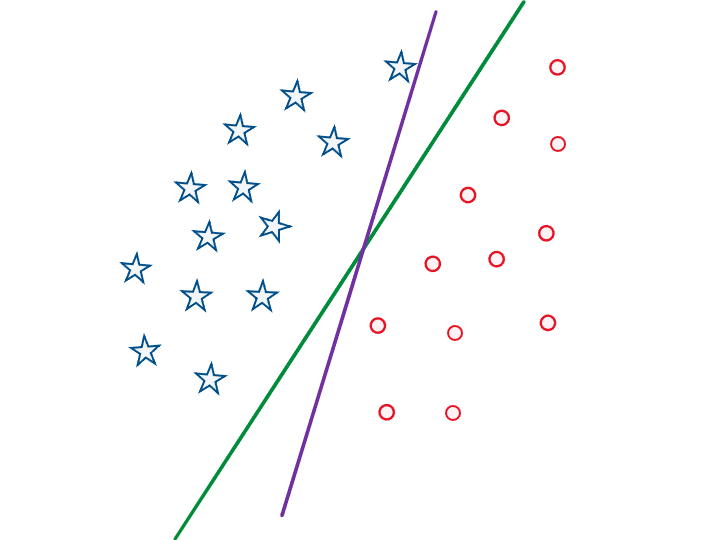
\includegraphics[height=6.5cm]{Figures/hyperplanes.png}
\caption{\label{fig:svm.1} 
The green line is preferable to the purple one in order to separate the data.
}
\end{figure} 


This leads to the maximum margin separating
hyperplane classifier, also called linear SVM, introduced by
Vapnik and Chervonenkis \cite{vapnik1998statistical,vapnik2013nature}.


\subsection{Maximizing the margin}
We will use the following result.
\begin{proposition}
\label{prop:dist.hyp}
The distance of a point $x\in\mR^d$ to the hyperplane $M: {a_0} + b^Tx = 0$ is given by $|{a_0} + x^Tb|/|b|$.
\end{proposition}
\begin{proof}
By definition, $\mathrm{distance}(x, M) = |x - \pi_M(x)|$ where $\pi_M$ is the orthogonal projection on $M$. 
Since $b$ is normal to $M$ and letting $h = \pi_M(x)$, we have $x = \la b + h$ so that  $|\la b| = \mathrm{distance}(x, M)$.
 Writing ${a_0} + b^T h = 0$ in this equation implies ${a_0} + b^T x = \la|b|^2$ so that $|\la|\, |b| = |{a_0} + x^Tb|/|b|$.
\end{proof}

 Assume that $T$ is linearly separable and let $M: {a_0} + b^Tx = 0$ be a separating hyperplane.
 The classification margin is defined as the minimal distance of the input vectors $x_1, \ldots, x_N$ to this hyperplane, i.e., 
\[
m({a_0}, b) = \min\{ |{a_0} + x_k^T b|/|b|: k=1, \ldots, N\}.
\]
 Because the hyperplane is separating, we have $y_k({a_0} + x_k^T b) = |{a_0} + x_k^T b|$ for all $k$, so that we also have
\[
m({a_0}, b) = \min\{ y_k({a_0} + x_k^T b)/|b|: k=1, \ldots, N\}.
\]
 We want to maximize this margin among all separating hyperplanes. This can be expressed as  maximizing, with respect to ${a_0}, b$, the quantity
\[
\min\{ y_k({a_0} + x_k^T b)/|b|: k=1, \ldots, N\}
\]
subject to the constraint that the hyperplane is separating, namely
\[
y_k({a_0} + x_k^T b) \geq 0,\ k=1, \ldots, N.
\]
Introducing a new variable $C$ representing the margin,  the previous problem is equivalent to maximizing $C$ subject to
\[
y_k({a_0} + x_k^T b) \geq C|b|,\ k=1, \ldots, N.
\]

The problem is now overparametrized, and there is no loss of generality in enforcing the additional constraint $C |b| = 1$. Noting that maximizing $C$ is the same as minimizing $|b|^2$, we can now reformulate the maximum margin hyperplane problem as minimizing $|b|^2/2$ subject to
\[
y_k({a_0} + x_k^T b) \geq 1,\ k=1, \ldots, N,
\]
with $C$ (the margin) given by $C = 1/|b|$.
 This results in a quadratic programming problem.

If the data is not separable, there is no feasible point for this problem. To also account for this situation (which is common), 
we can replace the constraint by a penalty and minimize, with respect to ${a_0}$ and  $b$:
\[
\frac{|b|^2}2 + \ga \sum_{k=1}^N (1 - y_k({a_0} + x_k^T b))^+
\]
for some $\ga >0$. (Recall that $x^+ = \max(x, 0)$.) This is equivalent to minimizing the perceptron objective function, with $\de=1$, and with an additional penalty term equal to $|b|^2/(2\ga)$. This minimization problem is equivalent to a quadratic programming problem obtained by introducing  slack variables $\xi_k$, $k=1, \ldots, N$ and  minimizing
\[
\frac{1}{2} |b|^2 + \ga \sum_{k=1}^N \xi_k\,,
\]
subject to the constraints $\xi_k \geq 0$, $y_k({a_0} + x_k^T b) + \xi_k
\geq 1$, for $k=1, \ldots, N$. 


\subsection{KKT conditions and dual problem}
Introduce Lagrange multipliers
$\eta_k\geq 0$ for $\xi_k \geq 0$ and $\al_k\geq 0$ for  $y_k({a_0} + x_k^T b) + \xi_k \geq 1$. 
The Lagrangian is then given by
$$
\mathcal L = \frac{1}{2} |b|^2 + \ga \sum_{k=1}^N \xi_k - \sum_{k=1}^N
\eta_k\xi_k -  \sum_{k=1}^N \al_k \big(y_k({a_0} + x_k^T b) +\xi_k - 1\big).
$$
The KKT conditions are
\begin{equation}
\label{eq:svm.kkt.class}
\left\{
\begin{aligned}
&b - \sum_{k=1}^N \al_k y_k x_k = 0\\
&\sum_{k=1}^N \al_k y_k = 0\\
& \ga - \eta_k - \al_k = 0,\quad  k=1, \ldots, N\\
& \xi_k\eta_k = 0, \quad k=1, \ldots, N\\
&  \al_k \big(y_k({a_0} + x_k^T b) +\xi_k - 1\big) = 0, \quad k=1, \ldots, N
\end{aligned}
\right.
\end{equation}

Minimizing $\mathcal L$ with respect to ${a_0}$, $b$ and $\xi_1, \ldots, \xi_N$ and ensuring that the minimum is finite provides the first three KKT conditions.
The resulting dual formulation therefore requires to
maximize
$$
\sum_{k=1}^N \al_k - \frac{1}{2} \sum_{k,l=1}^N \al_k\al_l y_ky_l x_k^Tx_l
$$
subject to the constraints $0\leq \al_k\leq \ga$, $\sum_{k=1}^N \al_k y_k =
0$. 

\bigskip
We now discuss the consequences of the complementary slackness conditions based on the position of training sample relative to the separating hyperplane.
\begin{enumerate}[label=(\roman*),wide=0cm] 
\item First consider indices $k$ such that $(x_k, y_k)$ is correctly classified {\em beyond the margin}, i.e., $y_k({a_0} + x_k^T b ) > 1$.
The last KKT condition and the constraint $\xi_k \geq 0$ require $\al_k = 0$, and the third one then gives $\xi_k=0$.
%\item This shows that such samples do not contribute to the solution. 
\item For samples that are misclassified or correctly classified below the margin
\footnote{Note that, even if the training data is linearly separable, there are generally samples that are on the right side of the hyperplane, but at a distance to the hyperplane strictly lower that the ``nominal margin'' $C = 1/|b|$. This is due to our relaxation of the original problem of finding a separating hyperplane with maximal margin.}, i,e.,  $y_k({a_0} + x_k^T b ) < 1$, the constraint $y_k({a_0} + x_k^Tb) +\xi_k \geq 1$ implies $\xi_k >0$, so that $\al_k = \ga$ and $y_k({a_0} + x_k^Tb) +\xi_k = 1$.
\item If $(x_k, y_k)$ is correctly classified exactly at the margin, then $\xi_k=0$ and there is no constrain on $\al_k$ beside belonging to $[0,\ga]$. 
Training samples that lie exactly at the margin are called \alert{support vectors}.
\end{enumerate}

Given a solution $\al_1, \ldots, \al_N$ of the dual problem, one immediately recovers $b$ via the first equation in \cref{eq:svm.kkt.class}. For ${a_0}$, one must, similarly to the regression case, rely on support vectors, which can be identified when $0 < \al_k < \ga$. In this case, one can take ${a_0} = y_k - x_k^T b$. 

If no support vector is found, then ${a_0}$ is not uniquely determined, and can be any value such that $y_k({a_0} + b^Tx_k) \geq 1$ if $\al_k=0$ and $y_k({a_0} + b^Tx_k) \leq 1$ if $\al_k = \ga$.  This shows that ${a_0}$ can be any point in the interval  $[\be^-_{0}, \be^+_{0}]$ with
\begin{align*}
&{a_0}^- =
\max\{ y_k- x_k^Tb: (y_k=1 \text{ and } \al_k=0) \text{ or } (y_k=-1 \text{ and } \al_k=\ga)\}  \\
&{a_0}^+ = \min\{ y_k- x_k^Tb: (y_k=-1 \text{ and } \al_k=0) \text{ or } (y_k=1 \text{ and } \al_k=\ga)\}.
\end{align*}


\subsection{Kernel version}
We make the usual assumptions: $h : \CR_X \to H$ is a feature map with values in an inner-product space with $K(x,y) = \scp{h(x)}{h(y)}_H$.  The predictors take the form $f(x) = \mathrm{sign}({a_0} + \scp{b}{h(x)}_H)$, ${a_0}\in \mR$ and $b\in H$,
and the goal is to minimize
\[
\frac{1}{2} \|b\|_H^2 + \ga \sum_{k=1}^N \xi_k\,,
\]
subject to $\xi_k \geq 0$, $y_k({a_0} + \scp{h(x_k)}{b}_H) + \xi_k \geq 1$, $k=1, \ldots, N$.

 Let $V = \vspan(h(x_1), \ldots, h(x_N))$. The usual projection argument implies that the optimal $b$ must belong to $V$ and therefore take the form
\[
b = \sum_{k=1}^N u_k h(x_k).
\]
We therefore need to minimize
\[
\frac{1}{2} \sum_{k,l=1}^N u_ku_l K(x_k, x_l) + \ga \sum_{k=1}^N \xi_k\,,
\]
subject to
\[
y_k\Big({a_0} + \sum_{l=1}^N K(x_k, x_l) a_l \Big)+ \xi_k
\geq 1
\]
for $k=1, \ldots, N$. Introducing the same Lagrange multipliers as before, the Lagrangian is 
\begin{multline*}
\CL = \frac{1}{2} \sum_{k,l=1}^N u_ku_l K(x_k, x_l) + \ga \sum_{k=1}^N \xi_k \\
- \sum_{k=1}^N
\eta_k\xi_k -  \sum_{k=1}^N \al_k \Big(y_k\Big({a_0} + \sum_{l=1}^N K(x_k, x_l) u_l\Big) +\xi_k - 1\Big)\,.
\end{multline*}
 Using vector notation, we have
\[
\CL = \frac12 u^T \CK u + \xi^T (\ga \dsone - \eta - \al) - {a_0} \al^T y - (\al\odot y)^T\CK u  + \al^T\dsone
\]
where $y\odot\al$ is the vector with coordinates $y_k\al_k$.
 The infimum of $\CL$ is $-\infty$ unless $\ga \dsone - \eta - \al=0$ and $\al^T y=0$.
 If these identities are true, then the optimal $u$ is $u = \al\odot y$ and the minimum of $\CL$ is
\[
- \frac12 (\al\odot y)^T\CK (\al\odot y)  + \al^T\dsone
\]

The dual problem therefore requires to minimize
\[
\frac12 (\al\odot y)^T\CK (\al\odot y)  - \al^T\dsone = \al^T(\CK\odot yy^T) \al  - \al^T\dsone
\]
subject to $\ga \dsone - \eta - \al=0$ and $\al^T y=0$.
\medskip

This is exactly the same problem as the one we obtained in the linear case, up to the replacement of the Euclidean inner products $x_k^Tx_l$ by the kernel evaluations $K(x_k, x_l)$. 
Given the solution of the dual problem, the optimal $b$ is 
\[
b=\sum_{k} u_k h(x_k) = \sum_{k=1}^N \al_k y_k h(x_k).
\]
It is no computable, but the classification rule is explicit and given by
\[
f(x) = \sign\left({a_0} + \sum_{k=1}^N \al_k y_k K(x_k,x)\right).
\]

Similarly to the linear case, the coefficient ${a_0}$ can be identified using a support vector, or is otherwise not uniquely determined. More precisely,  if one of the $\al_k$'s is strictly between $0$ and $\ga$, then ${a_0}$ is given by ${a_0} = y_k - \sum_l \al_l y_l K(x_k,x_l)$. Otherwise, ${a_0}$ is any number between 
\[
\be^-_{0} =
\max\defset{ y_k- \sum_l \al_l y_l K(x_k,x_l): (y_k=1 \text{ and } \al_k=0) \text{ or } (y_k=-1 \text{ and } \al_k=\ga)}  
\]
and 
\[
\be^+_{0} = \min\defset{ y_k- \sum_l \al_l y_l K(x_k,x_l):  (y_k=-1 \text{ and } \al_k=0)
 \text{ or } (y_k=1 \text{ and } \al_k=\ga)}.
\]
